\documentclass[lineno]{biometrika}

\usepackage{amsmath}
\usepackage{xcolor}
%\usepackage{graphics}
\usepackage{arydshln} % For \hdashline
\usepackage{array}    % For custom column types
\usepackage{booktabs} % For \toprule, \midrule, \bottomrule
\usepackage{longtable}

%% Please use the following statements for
%% managing the text and math fonts for your papers:
%\usepackage{times}
%\usepackage[cmbold]{mathtime}
%\usepackage{bm}
\usepackage[ruled,vlined,noend]{algorithm2e}

\usepackage{newtxtext}
\usepackage[subscriptcorrection]{newtxmath}

\newcommand{\blue}[1]{\textcolor{blue}{#1}}
\newcommand{\red}[1]{\textcolor{red}{#1}}
\definecolor{marooncustom}{rgb}{0.5, 0.0, 0.0}
\definecolor{ultramarine}{rgb}{0.07, 0.04, 0.56}
\newcommand{\tw}[1]{\textcolor{marooncustom}{(TW: #1)}}
\newcommand{\ek}[1]{\textcolor{ultramarine}{(EK: #1)}}
\definecolor{blue2}{rgb}{0.1, 0.2, 0.6}


%\usepackage{natbib}

\graphicspath{{./art/}}

\makeatletter
\renewcommand{\algocf@captiontext}[2]{#1\algocf@typo. \AlCapFnt{}#2} % text of caption
\renewcommand{\AlTitleFnt}[1]{#1\unskip}% default definition
\def\@algocf@capt@plain{top}
\renewcommand{\algocf@makecaption}[2]{%
\addtolength{\hsize}{\algomargin}%
\sbox\@tempboxa{\algocf@captiontext{#1}{#2}}%
\ifdim\wd\@tempboxa >\hsize%     % if caption is longer than a line
\hskip .5\algomargin%
\parbox[t]{\hsize}{\algocf@captiontext{#1}{#2}}% then caption is not centered
\else%
\global\@minipagefalse%
\hbox to\hsize{\box\@tempboxa}% else caption is centered
\fi%
\addtolength{\hsize}{-\algomargin}%
}
\makeatother

%%% User-defined macros should be placed here, but keep them to a minimum.
\def\Bka{{\it Biometrika}}
\def\AIC{\textsc{aic}}
\def\T{{ \mathrm{\scriptscriptstyle T} }}
\def\v{{\varepsilon}}

%\addtolength\topmargin{35pt}
\DeclareMathOperator{\Thetabb}{\mathcal{C}}
\newcommand{\simtableformat}{%
  \footnotesize
  \setlength{\tabcolsep}{3.5pt}%
  \renewcommand{\arraystretch}{0.95}%
}


\begin{document}

\jname{Biometrika}
%% The year, volume, and number are determined on publication
\jyear{2024}
\jvol{103}
\jnum{1}
\cyear{2024}
%% The \doi{...} and \accessdate commands are used by the production team
%\doi{10.1093/biomet/asm023}
\accessdate{Advance Access publication on 31 July 2023}

%% These dates are usually set by the production team
%\received{2 January 2017}
\revised{1 August 2023}

%% The left and right page headers are defined here:
\markboth{E. ZHU et~al.}{Biometrika style}

%% Here are the title, author names and addresses
\title{A fast simplex algorithm for local linear quantile regression}

\author{Erkang Zhu}
\affil{Department of Statistics and Data Science, Tsinghua University\\ Beijing, China 
\email{zek24@mails.tsinghua.edu.cn}}

\author{Tianying Wang}
\affil{Department of Statistics, Colorado State University\\ Fort Collins, CO, USA
\email{Tianying.Wang@colostate.edu}} %\thanks{Authors are listed in alphabetical order.}

\author{Weichi Wu}
\affil{Department of Statistics and Data Science, Tsinghua University\\ Beijing, China \email{wuweichi@tsinghua.edu.cn}\thanks{Corrsponding author: Weichi Wu (wuweichi@tsinghua.edu.cn).}}

\maketitle

\begin{abstract}
We study sequential kernel-weighted quantile regression problems arising in local linear quantile
regression and time-varying coefficient quantile regression. We propose an exact simplex-based
algorithm that combines warm starts, threshold-based screening and aggregation, and deterministic
verification. The verification step preserves the full LP solution in finite samples, while the
theory shows residual sign stability and shrinking screened problems under standard regularity
conditions. Simulations show substantial runtime gains relative to direct local fitting.
\end{abstract}

\begin{keywords}
Quantile regression.
\end{keywords}

\section{Introduction}\label{sec:intro}

Quantile regression models conditional quantiles and provides a robust alternative to least squares
when conditional distributions are heterogeneous or asymmetric (Koenker \& Bassett Jr, 1978).
Many quantile regression estimators can be computed by solving a linear program (LP), most commonly
via simplex type methods (Koenker \& d'Orey, 1987; Koenker, 2005) or interior point methods.

This paper focuses on \emph{local} and \emph{time-varying} quantile regression, where one must solve a
\emph{sequence} of closely related \emph{weighted} LPs across many evaluation points.
A canonical example is local linear quantile regression (LLQR) (Yu \& Jones, 1998), where at each location
$z$ one solves a kernel-weighted quantile regression. A second example is time-varying coefficient quantile
regression (TVCQR) (Wu \& Zhou, 2017), where coefficients evolve smoothly in time and are estimated by local
fitting. In both settings, evaluation is typically performed on a dense grid $\{s_j\}_{j=1}^m$ with $m$ comparable
to $n$. Naively, this requires solving $m$ weighted LPs, each with $n$ equality constraints and $2n$ nonnegative
slack variables. The computational burden is amplified in bootstrap based inference, where the full grid of fits
must be recomputed many times.

Warm starts can exploit similarity between neighboring evaluation points by reusing information from a nearby
solution, but they still operate on the full LP dimension at every point. There is also a literature on fast
computation for sequences of quantile regressions, including preprocessing ideas (Portnoy \& Koenker, 1997)
and fast algorithms for the quantile regression process indexed by the quantile level (Chernozhukov et al., 2020).
These methods primarily exploit stability as the quantile index varies under a fixed design and fixed observation
weights. In contrast, the local and time-varying problems considered here are indexed by \emph{location} (or time),
and the \emph{kernel weights vary with the index}. This changing objective structure motivates a reduction scheme
tailored to location-indexed sequences.

We propose an \emph{exact} screening and aggregation scheme for fast computation of kernel-weighted quantile
regressions on a grid. The key observation is that between adjacent evaluation points, fitted residuals typically
change little, so observations with residuals safely away from zero often keep the same sign. Conditional on correct
residual signs, the check loss is linear, and the contribution of all safely positive (respectively negative) residuals
can be represented exactly through one aggregated pseudo-observation. This yields a reduced LP involving only the
observations near the fitted quantile. Since sign stability can fail in finite samples, we add a verification step:
after solving the reduced LP, we check all omitted observations. Any violating observation is added back to the reduced
set and the reduced LP is re-solved. The reduced set grows monotonically and is bounded by $n$, hence the procedure
terminates after finitely many re-solves and returns the \emph{exact} solution of the full kernel-weighted LP for any
dataset. In the worst case the reduced set equals the full sample, so exactness is never traded for speed.

We solve the (full and reduced) LPs using simplex. Simplex is attractive here because its basis representation supports
effective warm starts across neighboring evaluation points, which often reduces pivot counts in practice when the
objective changes smoothly. We do not attempt to bound simplex pivot counts, which are difficult to characterize in
general. Instead, our theoretical analysis targets a solver-agnostic quantity: the dimension of the reduced LP.
Under standard smoothness assumptions, we show that residual signs are stable with probability tending to one and that
the reduced set is asymptotically negligible relative to the local effective sample size, yielding a provable reduction
in LP dimension. We establish analogous results for TVCQR.

We make three contributions. First, we give an exact screened and aggregated LP construction with a finite-sample
verification guarantee for location-indexed kernel-weighted quantile regression sequences. Second, we provide theory
showing that the reduced LP dimension is asymptotically negligible under smoothness, giving a provable reduction in LP
size independent of pivot-count analyses. Third, we illustrate the framework in LLQR and TVCQR and present numerical
results showing substantial speedups while matching baseline solutions to numerical tolerance. The main text focuses on
the core algorithm, its exactness mechanism, the main theory statements, the median-runtime comparison, and a brief
discussion of broader applicability. Additional algorithmic details and supplementary simulations are deferred to the
Appendix.

\section{Method}\label{sec:method}

\subsection{Problem setup and a fixed-constraint LP representation}

We start from a generic weighted quantile regression problem that covers both LLQR and TVCQR after a simple
reparameterization. Let $(y_i,d_i)\in\mathbb R\times\mathbb R^q$ for $i=1,\ldots,n$, where $d_i$ is a design vector and
$q$ is the parameter dimension. Let $w_i(s)\ge 0$ be a weight that depends on an evaluation index $s$. For a fixed
$\tau\in(0,1)$, define
\begin{equation}
\hat\theta(s)\in\arg\min_{\theta\in\mathbb R^q}\sum_{i=1}^n w_i(s) \rho_\tau \bigl(y_i-d_i^\top\theta\bigr),
\qquad
\rho_\tau(u)=u\{\tau-\mathbf 1(u<0)\}.
\label{eq:weighted-qr}
\end{equation}
Introduce slack variables $u_i=\max(y_i-d_i^\top\theta,0)$ and $v_i=\max(d_i^\top\theta-y_i,0)$ so that
$y_i-d_i^\top\theta=u_i-v_i$ with $u_i,v_i\ge 0$. Then \eqref{eq:weighted-qr} is equivalent to the LP
\begin{equation}
\min_{\theta,u,v} \tau\sum_{i=1}^n w_i(s)u_i + (1-\tau)\sum_{i=1}^n w_i(s)v_i,
\quad\text{s.t.}\quad
d_i^\top\theta+u_i-v_i=y_i,   u_i,v_i\ge 0.
\label{eq:full-lp}
\end{equation}
In our applications, after reparameterization the design vectors $d_i$ do not depend on $s$. Consequently, the constraint
matrix in \eqref{eq:full-lp} is fixed across evaluation points, and only the objective coefficients change through $w_i(s)$.
This fixed-constraint structure is the reason warm starts are effective and why screening can be analyzed cleanly.


\textbf{Local linear quantile regression (LLQR)}
Let $(X_i,Y_i)$ be i.i.d., with bandwidth $b_n>0$ and kernel $K$. At location $z$, LLQR solves
\begin{equation}\label{eq:LLQR}
    (\hat\beta_0(z),\hat\beta_1(z))\in
\arg\min_{\beta_0,\beta_1}\sum_{i=1}^n
K \left(\frac{X_i-z}{b_n}\right)\rho_\tau \bigl(Y_i-\beta_0-\beta_1(X_i-z)\bigr).
\end{equation}

With the reparameterization $\alpha_0(z)=\beta_0(z)-z\beta_1(z)$ and $\alpha_1(z)=\beta_1(z)$, this becomes
\begin{equation}
(\hat\alpha_0(z),\hat\alpha_1(z))\in
\arg\min_{\alpha_0,\alpha_1}\sum_{i=1}^n w_i(z) \rho_\tau \bigl(Y_i-\alpha_0-\alpha_1 X_i\bigr),
\qquad
w_i(z)=K \left(\frac{X_i-z}{b_n}\right),
\label{eq:llqr-reparam}
\end{equation}
which matches \eqref{eq:weighted-qr} with $q=2$, $d_i=(1,X_i)^\top$, and $\theta=(\alpha_0,\alpha_1)^\top$.
The local quantile estimate is $\hat q_\tau(z)=\hat\beta_0(z)=\hat\alpha_0(z)+z\hat\alpha_1(z)$.


\textbf{Time-varying coefficient quantile regression (TVCQR)}
Let $t_i=i/n\in[0,1]$ and $x_i\in\mathbb R^p$ (including an intercept), and consider $Q_\tau(y_i\mid x_i)=x_i^\top\beta_\tau(t_i)$
with $\beta_\tau(\cdot)$ smooth. At time $t$, the local linear TVCQR estimator solves
\begin{equation}\label{eq:TVCQR}
    (\hat\beta_0(t),\hat\beta_1(t))\in
\arg\min_{\beta_0,\beta_1\in\mathbb R^p}\sum_{i=1}^n
K \left(\frac{t_i-t}{h_n}\right)\rho_\tau \bigl(y_i-x_i^\top\beta_0-(t_i-t)x_i^\top\beta_1\bigr).
\end{equation}

With $\theta_0(t)=\beta_0(t)-t\beta_1(t)$ and $\theta_1(t)=\beta_1(t)$,
\[
y_i-x_i^\top\beta_0-(t_i-t)x_i^\top\beta_1
=
y_i-x_i^\top\theta_0-(t_i x_i)^\top\theta_1.
\]
Thus \eqref{eq:weighted-qr} holds with $q=2p$, $d_i=(x_i^\top,(t_i x_i)^\top)^\top$, and weights $w_i(t)=K((t_i-t)/h_n)$.
The one-dimensional procedure summarized in Algorithm~\ref{alg:exact-screened} therefore applies verbatim.

\subsection{Sequential computation on a grid: screening, aggregation, warm starts, and verification}

Let $s_1<\cdots<s_m$ be an ordered grid of evaluation points (for LLQR, $s_j=z_j$; for TVCQR, $s_j=t_j$). We compute
$\hat\theta(s_j)$ sequentially. Because the constraints in \eqref{eq:full-lp} are fixed across $s$, we can warm start simplex
at $s_{j+1}$ using basis information from $s_j$. Warm starts can reduce pivot counts substantially in practice, but our main,
provable speedup comes from reducing LP dimension via screening and aggregation.

Assume $\hat\theta(s_j)$ has been computed and define fitted residuals
\[
\hat e_i(s_j)=y_i-d_i^\top\hat\theta(s_j),\qquad i=1,\ldots,n.
\]
Choose a threshold $\gamma_n>0$ and define the partition
\begin{equation}
H_j=\{i:\hat e_i(s_j)>\gamma_n\},\qquad
L_j=\{i:\hat e_i(s_j)<-\gamma_n\},\qquad
S_j=\{i:|\hat e_i(s_j)|\le \gamma_n\}.
\label{eq:partition}
\end{equation}
The set $S_j$ is the \emph{uncertain set}. Observations in $H_j\cup L_j$ are predicted to keep the same residual sign at $s_{j+1}$.

Let $w_i=w_i(s_{j+1})$ denote the weights at the next evaluation point. Define aggregated quantities
\[
W_H=\sum_{i\in H_j} w_i,\qquad
\bar d_H=\frac{1}{W_H}\sum_{i\in H_j} w_i d_i,\qquad
\bar y_H=\frac{1}{W_H}\sum_{i\in H_j} w_i y_i,
\]
and similarly $(W_L,\bar d_L,\bar y_L)$ for $L_j$, omitting an aggregated row if the corresponding weight sum is zero.

We solve a reduced LP at $s_{j+1}$ that keeps individual constraints for $i\in S_j$ and replaces each sure-sign group by one
pseudo-observation. For $i\in S_j$, keep the usual slack pair $(u_i,v_i)$. For the positive-residual group, keep only $u_H\ge 0$
and impose $\bar d_H^\top\theta+u_H=\bar y_H$. For the negative-residual group, keep only $v_L\ge 0$ and impose
$\bar d_L^\top\theta-v_L=\bar y_L$. The reduced objective uses the group weights $W_H$ and $W_L$:
\begin{align}
\min_{\theta, u, v, u_H, v_L}  
& \tau\sum_{i\in S_j} w_i u_i + (1-\tau)\sum_{i\in S_j} w_i v_i
  + \tau W_H u_H + (1-\tau) W_L v_L, \label{eq:reduced-obj}\\
\text{s.t.}  
& d_i^\top\theta+u_i-v_i=y_i,\quad u_i,v_i\ge 0,\qquad i\in S_j, \label{eq:reduced-uncertain}\\
& \bar d_H^\top\theta+u_H=\bar y_H,\quad u_H\ge 0, \label{eq:reduced-H}\\
& \bar d_L^\top\theta-v_L=\bar y_L,\quad v_L\ge 0. \label{eq:reduced-L}
\end{align}
Using $\bar d_H,\bar y_H$ (and $\bar d_L,\bar y_L$) instead of unscaled sums improves numerical conditioning. Equivalently, one may
use unscaled sums and rescale the corresponding slack variables; the two formulations are algebraically equivalent.

\textbf{Exactness conditional on correct signs.}
If $y_i-d_i^\top\theta\ge 0$ for all $i\in H_j$ at the optimizer, then in the full LP \eqref{eq:full-lp} the optimal slacks satisfy
$v_i=0$ and $u_i=y_i-d_i^\top\theta$ for $i\in H_j$. Hence the contribution of $H_j$ to the objective equals
$\tau\sum_{i\in H_j} w_i\{y_i-d_i^\top\theta\}=\tau W_H\{\bar y_H-\bar d_H^\top\theta\}=\tau W_H u_H$,
with $u_H=\bar y_H-\bar d_H^\top\theta\ge 0$ enforced by \eqref{eq:reduced-H}. An analogous identity holds for $L_j$ under
$y_i-d_i^\top\theta\le 0$ for all $i\in L_j$. Thus, conditional on correct residual signs for the sure-sign groups, the reduced LP
\eqref{eq:reduced-obj}--\eqref{eq:reduced-L} is algebraically equivalent to the full LP at $s_{j+1}$.

\subsection{Verification, termination, and finite-sample exactness}

After solving the reduced LP at $s_{j+1}$ and obtaining $\tilde\theta(s_{j+1})$, we verify the sign assumptions by computing full
residuals $\tilde e_i=y_i-d_i^\top\tilde\theta(s_{j+1})$ for all $i\in H_j\cup L_j$:
\[
V_H=\{i\in H_j:\tilde e_i<0\},\qquad
V_L=\{i\in L_j:\tilde e_i>0\}.
\]
If $V_H\cup V_L$ is empty, then the sign conditions hold and the reduced LP is equivalent to the full LP, so
$\tilde\theta(s_{j+1})=\hat\theta(s_{j+1})$.

If violations occur, we move all violating indices into the uncertain set and re-solve:
\[
S_j\leftarrow S_j\cup V_H\cup V_L,\qquad
H_j\leftarrow H_j\setminus V_H,\qquad
L_j\leftarrow L_j\setminus V_L,
\]
then recompute the aggregates at $s_{j+1}$ and re-solve the reduced LP. This retry loop yields deterministic finite-sample exactness
because $S_j$ increases monotonically and is bounded by $\{1,\ldots,n\}$. Hence after finitely many re-solves, either no violations
remain or $S_j=\{1,\ldots,n\}$ and the reduced LP coincides with the full LP.

\textbf{Choice of $\gamma_n$.}
The threshold $\gamma_n$ controls the reduced LP dimension through $|S_j|$.
Section~\ref{sec:theory} provides sufficient asymptotic conditions on $\gamma_n$ for residual sign stability and a
bound on $|S_j|$.
In implementation we use a data-driven rule of the same asymptotic order; details are reported in the Supplementary Material.
Algorithm~\ref{alg:exact-screened} in Appendix~\ref{app:algorithms} summarizes the resulting one-dimensional procedure.

\subsection{Broader applicability beyond LLQR and TVCQR}\label{sec:broader}

Although we develop the method for LLQR and TVCQR, the screening, aggregation, and verification idea is not tied to
these two models. The key requirement is that, for each evaluation index $s$ on a dense grid, the estimator is defined
as the solution of a \emph{weighted} quantile regression problem with check loss,
\begin{equation}
\hat\theta(s)\in\arg\min_{\theta\in\mathbb R^q}\sum_{i=1}^n w_i(s)\,\rho_\tau\!\bigl(y_i-d_i(s)^\top\theta\bigr),
\qquad \rho_\tau(u)=u\{\tau-\mathbf 1(u<0)\},
\label{eq:generic_weighted_qr}
\end{equation}
so that each subproblem is a linear program. The aggregation step uses only the piecewise linearity of $\rho_\tau$:
if the residual sign of an observation is known at the optimizer, its contribution to the objective is linear in
$\theta$. Therefore, any collection of observations whose signs are correctly classified can be collapsed into two
pseudo-constraints, one for the positive-residual group and one for the negative-residual group, without changing the
optimization problem. The verification step then checks the omitted observations and deterministically repairs any
misclassification by moving violators into the retained set and re-solving. Consequently, finite-sample exactness is
preserved whenever the underlying estimator at each $s$ is defined by \eqref{eq:generic_weighted_qr} (or an equivalent
LP) and the verification step is implemented.

The most favorable setting for warm starts is when the dependence on $s$ enters only through the weights, so that after
a model-specific reparameterization the design vectors $d_i(s)$ become constant in $s$, yielding a fixed constraint
matrix across grid points. LLQR and TVCQR have exactly this structure, and the same mechanism appears in several other
quantile models that require fitting on a dense grid: (i) local polynomial quantile regression of order $r$, where
binomial expansion yields a fixed design $d_i=(1,X_i,\ldots,X_i^r)^\top$ and only kernel weights vary with $z$;
(ii) varying-coefficient quantile regression indexed by a scalar $Z_i$, where $x_i\in\mathbb R^p$ is a regressor
vector (including an intercept) and $Q_\tau(Y_i\mid x_i,Z_i=z)=x_i^\top\beta_\tau(z)$ with $\beta_\tau(\cdot)$ smooth;
(iii) partially linear and semiparametric quantile regression with a local component, where global coefficients enter
through additional fixed columns in $d_i$ and the local component is handled by kernel weights; (iv) local additive
quantile regression fitted by backfitting (Yu \& Lu, 2004), where each coordinate update requires solving many
one-dimensional local quantile regressions and the present method can accelerate each inner grid sweep; and
(v) locally weighted censored quantile regression (Wang \& Wang, 2009) and other locally weighted estimators, as long
as the estimator at each $s$ is still characterized by a weighted check-loss LP so that sign-based aggregation applies.

For extensions beyond LLQR and TVCQR, the deterministic verification step continues to guarantee exactness of each LP
solve, but the theoretical dimension reduction requires additional regularity conditions ensuring residual sign
stability between neighboring evaluation points. In our analysis this stability follows from smoothness of the target
quantile function, smooth variation of the weights, and dense evaluation grids. Analogous results can often be
obtained whenever a uniform Bahadur-type representation is available for the local quantile estimator and the grid
spacing is small relative to the smoothing scale, but the details depend on the specific model.

\medskip\noindent\textbf{Multivariate extension via a Euclidean minimum spanning tree.}
In one dimension the evaluation points are naturally ordered, so the procedure follows a forward sweep along the grid.
In higher dimensions there is no canonical linear order. A natural extension is to construct a Euclidean minimum
spanning tree on the evaluation points, choose a root, and process the nodes according to a tree traversal such as
Prim's growth order \cite{Prim1957}. Each non-root node is then paired with a parent node, and the exact solution and
basis at the parent can be used as a warm start for the child problem.

Under this traversal, the screened reduced LP at each child node is formed in the same way as in the one-dimensional
setting, using the parent solution to classify residual signs and initialize the simplex basis. The exact verification
step is unchanged: after solving the reduced LP at the child node, one checks the omitted observations, moves any
violators into the retained set, and re-solves until exactness is achieved. Thus the multivariate variant modifies only
the processing order and warm-start schedule, while leaving the reduction and verification mechanism unchanged. This
provides a natural multivariate analogue of the ordered one-dimensional sweep. A formal algorithm and supplementary
discussion are deferred to Appendix~\ref{app:mst}.

\section{Theory}\label{sec:theory}

We first introduce some notation. Let $\mathbf{1}(\cdot)$ be the indicator function. For a vector
$\mathbf{v}=(v_1,v_2\ldots,v_p)^\top\in\mathbb{R}^p$, let $|\mathbf{v}|=(\sum_{i=1}^pv_i^2)^{1/2}$. For a random
vector $\mathbf{V}$, write $\|\mathbf{V}\|_q=[\mathbb{E}|\mathbf{V}|^q]^{1/q}$ and $\|\mathbf{V}\|=\|\mathbf{V}\|_2$.
For a $p\times p$ matrix $V$, let $\lambda_{\max}(V)$ and $\lambda_{\min}(V)$ denote its largest and smallest
eigenvalues, respectively. Let the symbol $\lesssim$ mean ``left side bounded by a positive constant times the right
side'' (the symbol $\gtrsim$ is defined similarly). Since we consider estimation at a fixed $\tau$-level, we omit the
subscript $\tau$ when there is no ambiguity.

As discussed in Section~\ref{sec:method}, a naive approach solves, at each evaluation point $s_j$, a quantile
regression problem based on all $n$ observations with $q$ covariates (for example, $q=2p$ for TVCQR and $q=2$ for
univariate LLQR). Under a standard revised-simplex implementation, a single pivot costs $O(nq)$ operations.
Consequently, if $\kappa^{\mathrm{full}}_j$ denotes the data-dependent number of pivots required at $s_j$, then the
dominant pivoting cost of the baseline approach is on the order of
$O\!\big(q\sum_{j=1}^m \kappa^{\mathrm{full}}_j\,n\big)$.

Our sequential screening--aggregation algorithm reduces this cost by shrinking the problem size between adjacent
evaluation points. Given $\hat\theta_n(s_j)$, we compute residuals and partition the indices into $(H_j,L_j,S_j)$ as
in \eqref{eq:partition} using the threshold $\gamma_n$. At $s_{j+1}$ we solve a reduced quantile regression problem
built from the uncertain set $S_j$, together with at most two aggregated summary observations from $H_j$ and $L_j$.
Equivalently, the reduced LP has an effective sample size of order $|S_j|$. If $\kappa^{\mathrm{seq}}_j$ denotes the
number of pivots needed to solve this reduced problem at $s_{j+1}$ using a warm start from $s_j$, and $R_j\ge 1$
counts the number of verification-driven re-solves, then the dominant pivoting cost becomes
$O\!\big(q\sum_{j=1}^{m-1} R_j\,\kappa^{\mathrm{seq}}_j\,|S_j|\big)$, which is smaller than the baseline once
$|S_j|\ll n$. The next two theorems justify the two main ingredients behind this reduction: residual sign stability and
control of the size of the uncertain set.


\begin{condition}[Maximal spacing]\label{cond:spacing}
Let $\{s_1,\ldots,s_m\}\subset\mathcal A$ be ordered evaluation points (we suppress the dependence of $m$ on $n$).
Assume $\max_{1\le j\le m-1}|s_{j+1}-s_j|=O_{\mathbb P}(a_n)$ for some deterministic $a_n\to 0$.
\end{condition}

\begin{condition}[Coordinatewise uniform rates and smoothness]\label{cond:rate}
For each $k=1,\ldots,q$, there exists a bounded continuous function $\theta_k(\cdot):\mathcal A\to\mathbb R$ such that
$\sup_{s\in\mathcal A}|\hat\theta_{n,k}(s)-\theta_k(s)|=O_{\mathbb P}(\pi_{n,k})$ for some deterministic $\pi_{n,k}\to 0$ as $n\to\infty$.
Write $\theta(s)=(\theta_1(s),\ldots,\theta_q(s))^\top$.
Moreover, $\theta(\cdot)$ is Lipschitz on $\mathcal A$, i.e., $|\theta(s)-\theta(t)|\le L|s-t|$ for all $s,t\in\mathcal A$.
\end{condition}

\begin{condition}[Weight-induced neighborhood and regularity of regressors]\label{cond:reg}
Define the weight-induced neighborhood $\mathcal N_n(s)=\{i\in\{1,\ldots,n\}:w_{i,n}(s)>0\}$.
This is without loss of generality since indices outside $\mathcal N_n(s)$ have zero contribution to \eqref{eq:weighted-qr}.
Assume:
(i) for each $i$ and $k$, there exists a nonnegative random variable $C_{i,k}$ such that
$|d_{i,n,k}(s)-d_{i,n,k}(t)|\le C_{i,k}|s-t|$ for all $s,t\in\mathcal A$;
(ii) (coordinatewise bounds) there exist deterministic sequences $\{c'_{n,k}\}_{k=1}^q$ and $\{c_{n,k}\}_{k=1}^q$ such that
$\max_{1\le j\le m-1}\max_{i\in\mathcal N_n(s_j)} |d_{i,n,k}(s_j)|=O_{\mathbb P}(c'_{n,k})$ for all $k$ and
$\max_{1\le i\le n} C_{i,k}=O_{\mathbb P}(c_{n,k})$ for all $k$.
\end{condition}

\begin{condition}[Bounded conditional density]\label{cond:density}
Suppose there exists a filtration $\{\mathcal F_i\}_{i=1}^n$ such that
for each $i$, the conditional density $f(\cdot\mid\mathcal F_i)$ exists and there is a constant $M>0$ such that $\sup_{i\ge1}\ \sup_{y\in\mathbb R}\ f(y\mid\mathcal F_i)\le M$ almost surely.
\end{condition}


\begin{remark}
Condition~\ref{cond:spacing} ensures that the grid of evaluation points is sufficiently dense; intuitively, this suggests that the optimal solutions at adjacent points are close in an appropriate sense.
Condition~\ref{cond:rate} is a stability condition that typically follows from uniform convergence of the quantile estimator $\hat\theta_n(s)$; notably, the function $\theta(\cdot)$ need not coincide with the strict conditional quantile parameter in the sense of $Q_\tau(y_i\mid d_{i,n}(s))=d_{i,n}(s)^\top\theta(s)$.
Condition~\ref{cond:reg} characterizes the stochastic continuity of the regressors $d_{i,n}(\cdot)$ with respect to $s$ and controls their magnitudes on the relevant index set $\mathcal N_n(s)$ induced by the weights.
The uniform stochastic boundedness in Condition~\ref{cond:reg}(ii) typically holds under suitable moment or tail conditions on the regressors; for instance, in the TVCQR setting one may take $C_i=|x_i|$, and if the predictors $x_i$ are sub-Gaussian with uniformly bounded sub-Gaussian norms, then $c_n=\sqrt{\log n}$.
Combining Conditions~\ref{cond:spacing} and~\ref{cond:reg}(i) yields the uniform bound
$\max_{1\le j\le m-1}\max_{i\in\mathcal N_n(s_j)}|d_{i,n}(s_{j+1})-d_{i,n}(s_j)|=O_{\mathbb P}(c_n a_n)$.
\end{remark}

\begin{theorem}[Sign stability of the residuals]\label{thm:signstability}
Recall $\hat e_i(s)=y_i-d_{i,n}(s)^\top\hat\theta_n(s)$ and the partition
$H_j=\{i:\hat e_i(s_j)>\gamma_n\}$, $L_j=\{i:\hat e_i(s_j)<-\gamma_n\}$, $S_j=\{i:|\hat e_i(s_j)|\le \gamma_n\}$.
Suppose Conditions~\ref{cond:spacing}--\ref{cond:reg} hold. Define
$\bar S_{j,n}=\{i\in\mathcal N_n(s_j):|\hat e_i(s_j)|>\gamma_n\}=(H_j\cup L_j)\cap\mathcal N_n(s_j)$.
Let $\bar\pi_n=\sum_{k=1}^q \big[c^{\prime}_{n,k} \pi_{n,k}+ a_n c_{n,k} \pi_{n,k}+ a_n c_{n,k}+c_{n,k}^\prime\big]$.
Choose $\gamma_n=\bar\pi_n g_n$ with any $g_n\to\infty$ such that $\gamma_n\to 0$. Then, as $n\to\infty$,
\[
\mathbb P\big(\forall\,1\le j\le m-1,\ \forall\,i\in\bar S_{j,n}:\ \mathrm{sign}(\hat e_i(s_{j+1}))=\mathrm{sign}(\hat e_i(s_j))\big)\to 1.
\]
\end{theorem}

\noindent\emph{Proof.} The proof is given in the Appendix.

Theorem~\ref{thm:signstability} implies that, with probability tending to one, the screening step correctly predicts the residual signs from $s_j$ to $s_{j+1}$. Consequently, the reduced LP at $s_{j+1}$ is equivalent to the full LP in the sense that it recovers exactly the same optimizer, without requiring any sign-fixing corrections or threshold inflation (e.g., doubling the threshold). In this regime, the computational savings of our method come purely from solving a smaller LP obtained by dimension reduction. 


\begin{theorem}[Size of subsample]\label{thm:SizeOfSubsample}
Recall the partition \eqref{eq:partition} and note that
$|S_j|=\sum_{i=1}^n \mathbf 1\big(|\hat e_i(s_j)|\le \gamma_n\big)$ is the initial sample size at the evaluation point $s_{j+1}$ of the subsample chosen by the screening step.
Suppose Conditions~\ref{cond:spacing}--\ref{cond:density} hold and $\gamma_n$ is chosen as in Theorem~\ref{thm:signstability}.
Then, as $n\to\infty$,
\[
\max_{1\le j\le m-1}\ \mathbb E|S_j| = O(n\gamma_n).
\]
Here $|\cdot|$ denotes the cardinality of a set.
\end{theorem}

\noindent\emph{Proof.} The proof is given in the Appendix.

Theorem~\ref{thm:SizeOfSubsample} shows that the expected size of the uncertain set $S_j$ at any evaluation point is
small, in the sense that $\mathbb E|S_j|=O(n\gamma_n)$ uniformly over $j$. Since $\gamma_n\to 0$, the expected
subsample size constitutes a vanishing fraction of the full sample $n$. Moreover, under bounded kernel weights with
bandwidth $b_n$, the full LP at each $s_j$ effectively involves $O(n b_n)$ local constraints. If $\gamma_n=o(b_n)$,
then $\mathbb E|S_j|=o(n b_n)$, so our screening step reduces the expected LP size from order $n b_n$ to a strictly
smaller order.

The general conditions can be verified for LLQR and TVCQR under standard model-specific assumptions collected in the
Appendix. This yields the following corollaries.
\begin{corollary}[LLQR specialization]
\label{cor:llqr}
In the LLQR setting \eqref{eq:LLQR}, suppose Assumption~A1 in the Appendix holds.
Take the evaluation grid $s_j=X_{(j)}$ and choose the residual threshold
$\gamma_n=\bar\pi_n g_n$, where
$\bar\pi_n=(\frac{\log n}{nb_n})^{1/2}(1\vee \frac{a_n}{b_n})+a_n$ and $g_n=C\log\log n$ for $n\ge3$ and some constant $C>0$.
Then Theorems~\ref{thm:signstability} and~\ref{thm:SizeOfSubsample} apply to LLQR with residuals
$\hat e_i(s_j)=y_i-\hat\beta_0(s_j)-\hat\beta_1(s_j)(X_i-s_j)$.

In particular, the spacing term $a_n$ depends on the distribution of the design:
(i) if $X_i\stackrel{\mathrm{iid}}{\sim}U(0,1)$, then $a_n=\frac{\log n}{n}$, we can choose $\bar\pi_n=(\frac{\log n}{nb_n})^{1/2}$;
(ii) if $X_i\stackrel{\mathrm{iid}}{\sim}N(0,1)$, then $a_n=\frac{\log\log n}{\sqrt{\log n}}$, we can choose $\bar\pi_n=(\frac{1}{\sqrt{\log n}}+\frac{1}{\sqrt{nb_n^3}})\log\log n$.
\end{corollary}

\begin{corollary}[TVCQR specialization]
\label{cor:tvcqr}
In the TVCQR setting \eqref{eq:TVCQR}, suppose Assumption~A2 in the Appendix holds.
Take the evaluation grid $s_j=j/n$ and choose the residual threshold $\gamma_n=\bar\pi_n g_n$, where 
$\bar\pi_n=\frac{\log^{9/2} n}{(nb_n)^{1/2}}+b_n^2\log^{3/2} n$ and $g_n=C\log\log n$ for $n\ge 3$ and some constant $C>0$. 
Then Theorems~\ref{thm:signstability} and~\ref{thm:SizeOfSubsample} apply to TVCQR with residuals
$\hat e_i(s_j)=y_i-x_i^\top\hat\beta_0(s_j)-(i/n-s_j)x_i^\top\hat\beta_1(s_j)$.
\end{corollary}






\section{Simulation study}\label{sec:sim}

We consider four simulation settings. In Case~1, LLQR is fitted under a Gaussian design with
$X_i \stackrel{\mathrm{i.i.d.}}{\sim} N(0,1)$ and $y_i = 2X_i^2 + 1 + e_i$, where
$e_i \stackrel{\mathrm{i.i.d.}}{\sim} N(0,1)$. In Case~2, the same LLQR specification is used with
$X_i \stackrel{\mathrm{i.i.d.}}{\sim} U(0,1)$. In Case~3, TVCQR is fitted with
$x_{i,j}\stackrel{\mathrm{i.i.d.}}{\sim}N(0,1)$ for $j=1,2,3$ and
\[
y_i=\theta_0(i/n)+\theta_1(i/n)x_{i,1}+\theta_2(i/n)x_{i,2}+\theta_3(i/n)x_{i,3}+e_i,
\qquad e_i \stackrel{\mathrm{i.i.d.}}{\sim} N(0,1),
\]
where $\theta_0(t)=\sin(2\pi t)$, $\theta_1(t)\equiv 0.5$, $\theta_2(t)=2\log(1+2t)$, and
$\theta_3(t)=\exp\{-(t-0.5)^2\}$. Case~4 uses the same coefficient functions as Case~3, but generates the covariates
and errors from a locally stationary short-range dependent process; the detailed construction is given in
Appendix~\ref{app:supplement}. We consider sample sizes $n\in\{200,500,1000,2000,5000\}$ and $100$ Monte Carlo
replications per configuration. The main text focuses on $\tau=0.5$, while the additional results at
$\tau=0.2$ and $\tau=0.8$ are deferred to the Appendix.

Figure~\ref{fig:runtime_tau05_main} reports mean computation times at $\tau=0.5$ for
$n\in\{500,2000,5000\}$. To keep the main-text comparison compact, we display only three representative methods: the
baseline direct local fit (\texttt{llqr} in Cases~1--2 and \texttt{rq} in Cases~3--4), \texttt{seq(ft)}, and
\texttt{screen-seq(2)(ft)}. This reduced display separates the cost of direct local fitting, the effect of warm starts
under the faster implementation, and the additional effect of screening within the same implementation.

\begin{figure}[htbp]
\centering
\begin{minipage}{0.98\textwidth}
\centering
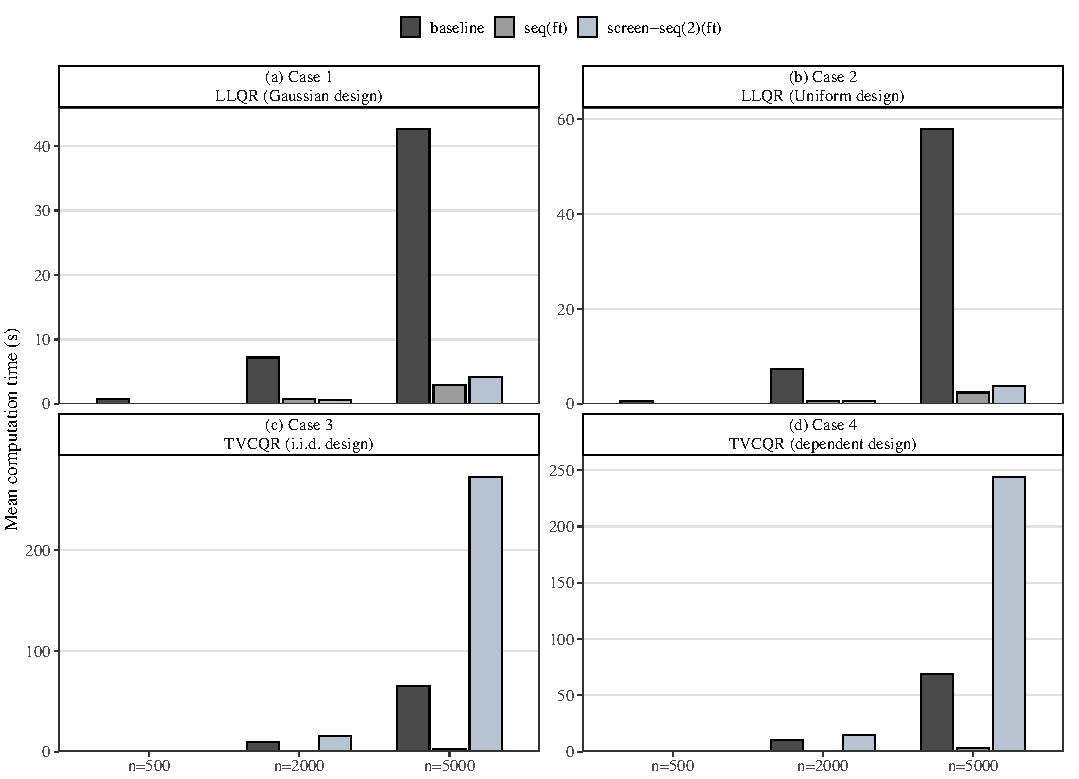
\includegraphics[width=\textwidth]{runtime_tau05_main}
\caption{Mean computation times at $\tau=0.5$ in the four simulation settings. Panels (a)--(d) correspond to
Case~1: LLQR (Gaussian design), Case~2: LLQR (Uniform design), Case~3: TVCQR (i.i.d. design), and
Case~4: TVCQR (dependent design). Only sample sizes $n=500,2000,5000$ are shown. The three displayed methods are the
baseline direct local fit, \texttt{seq(ft)}, and \texttt{screen-seq(2)(ft)}; the baseline corresponds to
\texttt{llqr} in Cases~1--2 and \texttt{rq} in Cases~3--4.}
\label{fig:runtime_tau05_main}
\end{minipage}
\end{figure}

Across all four cases, \texttt{seq(ft)} yields a substantial reduction in mean runtime relative to the baseline.
The comparison between \texttt{screen-seq(2)(ft)} and \texttt{seq(ft)} is more mixed. Screening can provide additional
reductions at some moderate sample sizes, but this advantage is not uniform and can reverse at the largest sample size
displayed. The overall pattern is consistent with warm starts providing the main computational gain, while the effect
of screening depends more strongly on the model setting.

Complete numerical summaries, including all reported methods, the ranges, and the results at $\tau=0.2$ and
$\tau=0.8$, are given in Appendix Table~\ref{tab:runtime_full}.


 

\bibliographystyle{biometrika}
\bibliography{paper-ref}

\newpage
\section{Appendix}\label{sec:appendix}

\subsection{Algorithmic summaries}\label{app:algorithms}

\begin{algorithm}[H]
\caption{Exact screened warm-start simplex on a grid}
\label{alg:exact-screened}
\DontPrintSemicolon
\KwIn{Ordered grid $s_1<\cdots<s_m$; data $(y_i,d_i)_{i=1}^n$; weights $w_i(s)$; quantile level $\tau$; threshold rule $\gamma_n$.}
\KwOut{Solutions $\hat\theta(s_j)$ for $j=1,\ldots,m$.}

Solve the full LP \eqref{eq:full-lp} at $s_1$ by simplex; store $\hat\theta(s_1)$ and an optimal basis $B_1$ 

\For{$j\gets 1$ \KwTo $m-1$}{
  Compute residuals $\hat e_i(s_j)=y_i-d_i^\top\hat\theta(s_j)$ for $i=1,\ldots,n$. 
  Form $(H_j,L_j,S_j)$ using \eqref{eq:partition} and threshold $\gamma_n$ 

  \Repeat{$V_H=\varnothing$ \textbf{and} $V_L=\varnothing$}{
    Compute aggregates at $s_{j+1}$ using weights $w_i(s_{j+1})$ 
    Build the reduced LP \eqref{eq:reduced-obj}--\eqref{eq:reduced-L} at $s_{j+1}$. 
    Solve the reduced LP by simplex, warm started from $B_j$ when possible; obtain $(\tilde\theta,\tilde B)$ 

    Compute $\tilde e_i=y_i-d_i^\top\tilde\theta$ for all $i\in H_j\cup L_j$. 
    Set $V_H=\{i\in H_j:\tilde e_i<0\}$ and $V_L=\{i\in L_j:\tilde e_i>0\}$ 

    \If{$V_H\neq\varnothing$ \textbf{or} $V_L\neq\varnothing$}{
      $S_j \gets S_j\cup V_H\cup V_L$ 
      $H_j \gets H_j\setminus V_H$ 
      $L_j \gets L_j\setminus V_L$ 
    }
  }

  $\hat\theta(s_{j+1})\gets \tilde\theta$; \quad $B_{j+1}\gets \tilde B$ 
}
\end{algorithm}

\subsection{Proofs of the main theorems}\label{app:proofs}

\begin{proof}[Proof of Theorem~\ref{thm:signstability}]
Write $\max_{ij}=\max_{1\le j\le m-1}\max_{i\in\mathcal N_n(s_j)}$ for short and define
$\mathcal E_n=\{\max_{ij}|\hat e_i(s_{j+1})-\hat e_i(s_j)|\le \gamma_n\}$.
On $\mathcal E_n$, if $|\hat e_i(s_j)|>\gamma_n$ then $\hat e_i(s_{j+1})$ cannot cross zero, hence
$\mathrm{sign}(\hat e_i(s_{j+1}))=\mathrm{sign}(\hat e_i(s_j))$ for all $i\in\bar S_{j,n}$ and all
$j\in\{1,\ldots,m-1\}$. It suffices to show $\mathbb P(\mathcal E_n)\to 1$.

Fix $j$ and $i\in\mathcal N_n(s_j)$. A direct decomposition yields
\begin{align*}
\hat e_i(s_{j+1})-\hat e_i(s_j)
=&\ d_{i,n}(s_j)^\top\bigl\{(\hat\theta_n(s_j)-\theta(s_j))-(\hat\theta_n(s_{j+1})-\theta(s_{j+1}))\bigr\}\\
&+\ (d_{i,n}(s_j)-d_{i,n}(s_{j+1}))^\top(\hat\theta_n(s_{j+1})-\theta(s_{j+1}))\\
&+\ d_{i,n}(s_j)^\top(\theta(s_j)-\theta(s_{j+1}))\\
&+\ (d_{i,n}(s_j)-d_{i,n}(s_{j+1}))^\top\theta(s_{j+1})\\
=&:\ I_1+I_2+I_3+I_4.
\end{align*}
By Conditions~\ref{cond:rate} and~\ref{cond:reg}(ii),
\[
\max_{ij}|I_1|
\le 2\sum_{k=1}^q \max_{ij}|d_{i,n,k}(s_j)|\,\sup_{s\in\mathcal A}|\hat\theta_{n,k}(s)-\theta_k(s)|
=O_{\mathbb P}\Big(\sum_{k=1}^q c^{\prime}_{n,k}\pi_{n,k}\Big).
\]
By Conditions~\ref{cond:reg}(i) and~\ref{cond:spacing},
\[
\max_{ij}|I_2|
\le \sum_{k=1}^q \max_i C_{i,k}\,\max_j|s_{j+1}-s_j|\,\sup_{s\in\mathcal A}|\hat\theta_{n,k}(s)-\theta_k(s)|
=O_{\mathbb P}\Big(a_n\sum_{k=1}^q c_{n,k}\pi_{n,k}\Big).
\]
By the Lipschitz property of $\theta(\cdot)$ and Condition~\ref{cond:reg}(ii),
$\max_{ij}|I_3|=O_{\mathbb P}\big(a_n\sum_{k=1}^q c_{n,k}^\prime\big)$.
Finally, using Condition~\ref{cond:reg}(i) and boundedness of $\theta(\cdot)$,
$\max_{ij}|I_4|=O_{\mathbb P}\big(a_n\sum_{k=1}^q c_{n,k}\big)$.
Therefore,
\[
\max_{ij}|\hat e_i(s_{j+1})-\hat e_i(s_j)|
=O_{\mathbb P}\Big(\sum_{k=1}^q\big[c^{\prime}_{n,k}\pi_{n,k}+a_n c_{n,k}\pi_{n,k}+a_n(c_{n,k}+c_{n,k}^\prime)\big]\Big)
=O_{\mathbb P}(\bar\pi_n).
\]
Since $\gamma_n=\bar\pi_n g_n$ with $g_n\to\infty$, we obtain
$\mathbb P(\mathcal E_n^c)=\mathbb P(\max_{ij}|\hat e_i(s_{j+1})-\hat e_i(s_j)|>\gamma_n)\to 0$.
\end{proof}

\begin{proof}[Proof of Theorem~\ref{thm:SizeOfSubsample}]
Fix $j\in\{1,\ldots,m-1\}$. By definition,
\[
\mathbb E|S_j|=\sum_{i=1}^n \mathbb P\big(|\hat e_i(s_j)|\le \gamma_n\big)
=\sum_{i=1}^n \mathbb P\big(|y_i-d_{i,n}(s_j)^\top\hat\theta_n(s_j)|\le \gamma_n\big).
\]
For each $i$, let $T_{i,j}:=d_{i,n}(s_j)^\top\hat\theta_n(s_j)$. Using
$\mathbb P(A)=\mathbb E[\mathbb P(A\mid T_{i,j})]$, we have
\[
\mathbb P\big(|y_i-T_{i,j}|\le \gamma_n\big)
=\mathbb E\Big[\mathbb P\big(|y_i-t|\le \gamma_n\big)\Big|_{t=T_{i,j}}\Big]
\le \sup_{t\in\mathbb R}\mathbb P\big(|y_i-t|\le \gamma_n\big).
\]
For any fixed $t\in\mathbb R$, Condition~\ref{cond:density} implies
\[
\mathbb P\big(|y_i-t|\le \gamma_n\mid \mathcal F_i\big)
=\int_{t-\gamma_n}^{t+\gamma_n} f(y\mid \mathcal F_i)\,dy
\le 2M\gamma_n\quad \text{a.s.},
\]
hence $\mathbb P(|y_i-t|\le \gamma_n)\le 2M\gamma_n$. Taking $\sup_t$ preserves the bound, so
$\mathbb P(|y_i-T_{i,j}|\le \gamma_n)\le 2M\gamma_n$ for all $i$ and $j$. Therefore,
\[
\mathbb E|S_j|\le \sum_{i=1}^n 2M\gamma_n = 2Mn\gamma_n,
\]
and taking $\max_{1\le j\le m-1}$ completes the proof.
\end{proof}

\subsection{Model-specific regularity conditions}\label{app:model-conditions}

\noindent\textbf{LLQR.}
\textit{Assumption A1.}

(\romannumeral1) $q_\tau(z)\in \mathcal{C}^3(\mathcal{X})$ where $\mathcal{X}$ is the support of $X$. $d^2 q_\tau(z)/d z^2$
is bounded with bounded first order derivatives.

(\romannumeral2) The distribution of $X$ has a strictly positive and continuously differentiable probability density
function $f(x)$ on $\mathbb{R}$.

(\romannumeral3) The conditional distribution of $Y$ given $X$ has a bounded, Lipschitz continuous density
$f(y|x)=\partial F(y|x)/\partial y$ in the sense that $|f(y|X)-f(y^\prime|X)|\le C|y-y^\prime|\ \text{a.s.}$ for some
constant $C>0$. Moreover, $\inf_{(x,y)\in\mathcal{X}\times\mathbb{R}}f(y|x)\ge\eta>0$ for some positive constant
$\eta$.

(\romannumeral4) The kernel function $K(\cdot)$ is nonnegative, symmetric and Lipschitz continuous over a compact
support $\mathcal{K}=[-1,1]$.

(\romannumeral5) The bandwidth $b_n$ satisfies $b_n\to 0$, $nb_n/\log n\to \infty$, and $nb_n^5/\log n\to 0$.

\begin{remark}
We specialize the assumptions from \cite{kong2010uniform} to the i.i.d.\ case, a restriction needed to ensure uniform
control over the maximal spacing of the evaluation points. The correspondence between their assumptions and ours is as
follows. Assumptions [A1] and [A2] of \cite{kong2010uniform} are readily satisfied by the check function
$\rho_\tau(x)$ and the error term $e_\tau=Y-q_\tau(X)$. Their Assumptions [A3] and [A5] correspond directly to
(\romannumeral4) and (\romannumeral1), respectively. The remaining assumptions follow from our framework: [A4] follows
from (\romannumeral2), [A6] (with $\lambda_2=1/2$) from (\romannumeral5), and [A7] from (\romannumeral2) and
(\romannumeral3).
\end{remark}

In LLQR, take $s_j=X_{(j)}$, where $X_{(1)}\le\cdots\le X_{(n)}$ are the order statistics of $X_1,\ldots,X_n$.
With a compactly supported kernel $K$ and bandwidth $b_n$, the weights have the form $w_{i,n}(s)=K((X_i-s)/b_n)$, so
$\mathcal N_n(s)=\{i:|X_i-s|\le b_n\}$ and Condition~\ref{cond:reg} is imposed only on this local window. The
local-linear design is $d_{i,n}(s)=(1,X_i-s)^\top$, so one may take $C_{i,1}=0$ and $C_{i,2}=1$ in
Condition~\ref{cond:reg}(i). Moreover, for $i\in\mathcal N_n(s)$ we have $|d_{i,n,1}(s)|=1$ and
$|d_{i,n,2}(s)|\le b_n$, hence $c'_{n,1}=1$ and $c'_{n,2}=b_n$ in Condition~\ref{cond:reg}(ii), while
$c_{n,1}=0$ and $c_{n,2}=1$.

Uniform LLQR theory (e.g., \cite{kong2010uniform}) provides the coordinatewise rates in Condition~\ref{cond:rate};
typically, $\pi_{n,1}= (\frac{\log n}{n b_n})^{1/2}$ and $\pi_{n,2}= \pi_{n,1}/b_n$ under standard bandwidth choices.
Thus we can take $\bar\pi_n=\pi_{n,1}(1\vee \frac{a_n}{b_n})+a_n$. Condition~\ref{cond:spacing} holds with $a_n$ given
by maximal spacing results for order statistics; for example, \cite{deheuvels1984strong} shows that if $X_i$ takes
values in a bounded support, then under suitable regularity conditions,
\[
\max_{1\le i\le n-1}\big|X_{(i+1)}-X_{(i)}\big|=O_{\mathrm{a.s.}}\!\big(\tfrac{\log n}{n}\big).
\]
Moreover, when $X_i\stackrel{\mathrm{iid}}{\sim}N(0,1)$, \cite{deheuvels1985limiting} establishes the bound
\[
\max_{1\le i\le n-1}\big|X_{(i+1)}-X_{(i)}\big|
=O_{\mathrm{a.s.}}\!\big(\tfrac{\log\log n}{\sqrt{\log n}}\big).
\]

\noindent\textbf{TVCQR.}
\textit{Assumption A2.}

Assume Assumptions [A0]--[A4] of \cite{wu2017nonparametric} hold, and $b_n\to 0$,
$nb_n^4/\log^7 n\to \infty$.

In TVCQR, take the equally spaced grid $s_j=t_j=j/n$, so $a_n=1/n$. Let
$\mathbf x_i=\mathbf H(i/n,\mathcal G_i)$ and consider the model $y_i=\beta(i/n)^\top\mathbf x_i+e_i$ at quantile
level $\tau$. With a compactly supported kernel $K$ and bandwidth $b_n$, the weights can be written as
$w_{i,n}(s)=K((i/n-s)/b_n)$, hence $\mathcal N_n(s)=\{i:|(i/n-s)/b_n|\le 1\}$. The local-linear design has the form
$d_{i,n}(s)=(\mathbf x_i^\top,\ \mathbf x_i^\top(i/n-s))^\top\in\mathbb R^{2p}$. Then for each coordinate in the first
block one has $|d_{i,n,k}(s)|\le |\mathbf x_i|$, while for each coordinate in the second block one has
$|d_{i,n,k}(s)|\le |\mathbf x_i||i/n-s|\le b_n|\mathbf x_i|$ on $\mathcal N_n(s)$. Moreover,
$|d_{i,n,k}(s)-d_{i,n,k}(t)|\le |\mathbf x_i||s-t|$ for coordinates in the second block and is zero for the first
block, so one may take $C_{i,k}= |\mathbf x_i|$ for the second block and $C_{i,k}=0$ for the first block.

If $|\mathbf x_i|$ is sub-Gaussian with uniformly bounded sub-Gaussian norms, then
$\max_{1\le i\le n}|\mathbf x_i|=O_{\mathbb P}(\sqrt{\log n})$, and hence one may take
$c'_{n,k}=O(\sqrt{\log n})$ for the first block, $c'_{n,k}=O(b_n\sqrt{\log n})$ for the second block, and
$c_{n,k}=O(\sqrt{\log n})$ for the second block. Lemma~3 of \cite{wu2017nonparametric} implies the uniform estimation
rates in Condition~\ref{cond:rate}; in particular, the first block satisfies
$\pi_{n,k}= (n b_n)^{-1/2}\log^4 n+b_n^2\log n$, and the second block typically satisfies
$\pi_{n,k}= ((n b_n)^{-1/2}\log^4 n+b_n^2\log n)/b_n$. Thus we can take
$\bar\pi_n=(nb_n)^{-1/2}\log^{9/2}n+b_n^2\log^{3/2}n$.

\subsection{Multivariate extension via a Euclidean minimum spanning tree}\label{app:mst}

Consider evaluation points $\{s_1,\ldots,s_m\}\subset \mathcal A\subset \mathbb R^r$ with $r\ge 2$. Let $T_m$ denote
the Euclidean minimum spanning tree on these points. Write $\bar s=m^{-1}\sum_{j=1}^m s_j$, and choose as root the
evaluation point closest to $\bar s$, breaking ties arbitrarily. To avoid conflict with the quantile level $\tau$, let
$\sigma(1),\ldots,\sigma(m)$ denote the growth order produced by Prim's algorithm started from this root
\cite{Prim1957}, and let $\pi(\sigma(\ell))$ denote the parent of $\sigma(\ell)$ in the rooted tree for
$\ell=2,\ldots,m$. Each non-root node corresponds to one parent--child edge, so
\[
\max_{2\le \ell\le m}\|s_{\sigma(\ell)}-s_{\pi(\sigma(\ell))}\|
\]
is the maximum parent--child edge length, equivalently the longest edge length of the rooted MST. The exact
verification step used in Algorithm~\ref{alg:exact-screened} is unchanged; only the processing order and warm-start
schedule are modified.

\begin{algorithm}[t]
\caption{Exact screened warm-start simplex on a multivariate grid via an MST}
\label{alg:mst-screened}
\DontPrintSemicolon
\KwIn{Evaluation points $\{s_1,\ldots,s_m\}\subset \mathcal A\subset \mathbb R^r$; data $(y_i,d_i)_{i=1}^n$; weights $w_i(s)$; quantile level $\tau$; threshold rule $\gamma_n$.}
\KwOut{Solutions $\hat\theta(s_j)$ for $j=1,\ldots,m$.}

Construct the Euclidean MST $T_m$ on $\{s_1,\ldots,s_m\}$.
Choose a root $\sigma(1)$ and obtain the rooted tree, the Prim growth order $\sigma(1),\ldots,\sigma(m)$, and the
parent map $\pi$ 

Solve the full LP \eqref{eq:full-lp} at $s_{\sigma(1)}$ by simplex; store $\hat\theta(s_{\sigma(1)})$ and an optimal
basis $B_{\sigma(1)}$ 

\For{$\ell\gets 2$ \KwTo $m$}{
  $u\gets \pi(\sigma(\ell))$; \quad $v\gets \sigma(\ell)$ 
  Compute parent residuals $\hat e_i(s_u)=y_i-d_i^\top\hat\theta(s_u)$ for $i=1,\ldots,n$ 
  Form $(H,L,S)$ from $\hat e_i(s_u)$ using \eqref{eq:partition} and threshold $\gamma_n$ 

  \Repeat{$V_H=\varnothing$ \textbf{and} $V_L=\varnothing$}{
    Compute aggregates at $s_v$ using weights $w_i(s_v)$ 
    Build the reduced LP \eqref{eq:reduced-obj}--\eqref{eq:reduced-L} at $s_v$ from $(H,L,S)$ 
    Solve the reduced LP by simplex, warm started from the exact parent basis $B_u$ on the first pass and from the
    current basis thereafter; obtain $(\tilde\theta,\tilde B)$ 

    Compute $\tilde e_i=y_i-d_i^\top\tilde\theta$ for all $i\in H\cup L$ 
    Set $V_H=\{i\in H:\tilde e_i<0\}$ and $V_L=\{i\in L:\tilde e_i>0\}$ 

    \If{$V_H\neq\varnothing$ \textbf{or} $V_L\neq\varnothing$}{
      $S \gets S\cup V_H\cup V_L$ 
      $H \gets H\setminus V_H$ 
      $L \gets L\setminus V_L$ 
    }
  }

  $\hat\theta(s_v)\gets \tilde\theta$; \quad $B_v\gets \tilde B$ 
}
\end{algorithm}

We record the following standard bound for the maximum parent--child edge length in a Euclidean MST; see
\cite{Penrose1997LongestEdgeMST,Penrose2003RGG}.

\begin{lemma}[Maximum parent--child edge length in a Euclidean MST]
Let $X_1,\ldots,X_n$ be i.i.d.\ random vectors in $\mathbb R^d$, where $d\ge 2$, with compact connected support
$\mathcal A$. Assume that the sampling density $f$ is continuous on $\mathcal A$ and bounded away from zero. Assume
further that either $\mathcal A=\mathbb T^d$ or $\mathcal A$ has $C^2$ boundary. Let $T_n$ be the Euclidean minimum
spanning tree on $\{X_i\}_{i=1}^n$, rooted arbitrarily, and let $\pi$ denote the parent map induced by the rooted
tree. If $v_0$ denotes the root, then
\[
\sup_{v\neq v_0}\|X_v-X_{\pi(v)}\| = O_{\mathbb P}\Bigl(\Bigl(\frac{\log n}{n}\Bigr)^{1/d}\Bigr).
\]
\end{lemma}

The left-hand side equals the longest edge length of the rooted MST.

The lemma indicates that, under standard random-design conditions, adjacent parent--child nodes in the MST are
uniformly close. This makes the exact solution at the parent node a plausible warm start for the child problem. For
this reason, the MST traversal provides a natural multivariate analogue of the one-dimensional ordered sweep, although
the present discussion is only heuristic and supplementary.

To check whether this heuristic is computationally useful in practice, we ran a supplementary multivariate LLQR
experiment with $p=4$, $\tau=0.5$, and evaluation points $z_i=x_i$. We compared the cold-start implementation
(\texttt{cold}), which solves each local LP from scratch, with the multivariate warm-start implementation
(\texttt{seq-MST}), which traverses the evaluation points in rooted MST order. In the implementation, the MST is
built after coordinatewise bandwidth normalization, so that geometric closeness better matches closeness of the kernel
weights. We considered two designs with $n\in\{300,500,800\}$ and $10$ Monte Carlo replications per configuration.
Case~1 uses i.i.d.\ Gaussian covariates together with a nonlinear regression surface and $t_4$ noise, whereas Case~2
uses correlated Gaussian covariates, a nonlinear mean function, and heteroskedastic Gaussian noise. In all runs, the
MST warm-started solutions agreed with the cold-start solutions up to numerical precision, with maximum absolute
discrepancy $1.18\times 10^{-12}$.

\begin{table}[htbp]
\centering
\caption{Mean total simplex iterations in the multivariate LLQR experiment with $p=4$, $\tau=0.5$, and $z_i=x_i$.
The last column reports the average percentage reduction in total iterations for \texttt{seq-MST} relative to
\texttt{cold}.}
\begingroup
\simtableformat
\begin{tabular}{rrrrr}
\toprule
Case & $n$ & cold & seq-MST & MST vs.\ cold \\
\midrule
1 & 300 & 66,505 & 21,869 & 67.1\% \\
1 & 500 & 175,608 & 53,559 & 69.4\% \\
1 & 800 & 446,355 & 124,175 & 72.2\% \\
2 & 300 & 49,061 & 15,630 & 68.1\% \\
2 & 500 & 133,264 & 36,897 & 72.3\% \\
2 & 800 & 341,006 & 86,155 & 74.7\% \\
\bottomrule
\end{tabular}
\endgroup
\label{tab:mst_multivar_iterations}
\end{table}

\texttt{seq-MST} consistently reduces total iterations by roughly two thirds or more, with reductions of
$67.1\%$--$72.2\%$ in Case~1 and $68.1\%$--$74.7\%$ in Case~2. Averaged over all runs, the mean parent--child edge
length under the bandwidth-scaled MST traversal was $0.91$. These calculations support the heuristic that, in higher
dimensions, an MST traversal supplies a substantially local warm-start schedule and can sharply reduce the number of
simplex pivots relative to solving each local problem from scratch.

\subsection{Supplementary simulation details}\label{app:supplement}

\noindent\textbf{Additional details for TVCQR (dependent design).}
To move beyond the i.i.d.\ design in Section~\ref{sec:sim}, we also consider a locally stationary short-range
dependent TVCQR setting adapted from Wu \& Zhou (2017). Let $t_i=i/n$ and define
\[
a(t)=\frac{1}{2}-\Bigl(t-\frac{1}{2}\Bigr)^2,\qquad
b(t)=\frac{1}{2}-\frac{t}{2},\qquad
c(t)=\frac{1}{4}+\frac{t}{2}.
\]
We generate
\[
e_i=e(t_i),\qquad e(t)=\sum_{j=0}^\infty a(t)^j\zeta_{i-j}/4,
\]
\[
x_{i,1}=x_{i,1}(t_i),\qquad x_{i,1}(t)=\sum_{j=0}^\infty b(t)^j\xi_{i-j},
\]
\[
x_{i,2}=x_{i,2}(t_i),\qquad x_{i,2}(t)=\sum_{j=0}^\infty c(t)^j\eta_{i-j},
\]
where $\xi_i=(\eta_i+\varepsilon_i)/\sqrt{2}$ and $\{\zeta_i\}$, $\{\eta_i\}$, and $\{\varepsilon_i\}$ are mutually
independent i.i.d.\ $N(0,1)$ sequences. To match the three-covariate specification in the i.i.d.\ TVCQR design, we further let
\[
x_{i,3}\stackrel{\mathrm{i.i.d.}}{\sim}\chi_3^2/3
\]
independently of the innovation sequences, and generate
\[
y_i=\theta_0(t_i)+\theta_1(t_i)x_{i,1}+\theta_2(t_i)x_{i,2}+\theta_3(t_i)x_{i,3}+e_i,
\]
with the same coefficient functions as in the i.i.d.\ TVCQR design,
\[
\theta_0(t)=\sin(2\pi t),\qquad
\theta_1(t)\equiv 0.5,\qquad
\theta_2(t)=2\log(1+2t),\qquad
\theta_3(t)=\exp\{-(t-0.5)^2\}.
\]
Then
\[
Q_\tau(y_i\mid x_i)=\theta_0(t_i)+\theta_1(t_i)x_{i,1}+\theta_2(t_i)x_{i,2}+\theta_3(t_i)x_{i,3}+e_{i,\tau},
\]
where $e_{i,\tau}$ denotes the $\tau$-quantile of $e_i$. In implementation, the infinite sums are replaced by
sufficiently long truncated filters with burn-in, and we use the same sample sizes, bandwidth rule, evaluation grid,
and reporting convention as in the i.i.d.\ TVCQR design.

The complete runtime summaries for Cases~1--4, all reported methods, and $\tau\in\{0.2,0.5,0.8\}$ are collected in
Table~\ref{tab:runtime_full}. Any numerical illustration of the MST-sequential variant remains supplementary and is not
developed as a main empirical contribution.

\subsection{Complete runtime summaries}\label{app:runtime}

Table~\ref{tab:runtime_full} reports the full runtime results for all four cases, all reported methods, and all sample
sizes. Each entry records the Monte Carlo mean computation time together with the range (max--min).

\begingroup
\scriptsize
\setlength{\tabcolsep}{2.8pt}
\renewcommand{\arraystretch}{0.95}
\begin{longtable}{lllrrrrrrrrrr}
\caption{Complete runtime summaries for the four simulation settings. Case~1 = LLQR (Gaussian design), Case~2 = LLQR (Uniform design), Case~3 = TVCQR (i.i.d. design), and Case~4 = TVCQR (dependent design). Entries report the Monte Carlo mean computation time and range (max--min), in seconds, over $100$ replications.}\label{tab:runtime_full}\\
\toprule
Case & $\tau$ & Method & \multicolumn{2}{c}{$n=200$} & \multicolumn{2}{c}{$n=500$} & \multicolumn{2}{c}{$n=1000$} & \multicolumn{2}{c}{$n=2000$} & \multicolumn{2}{c}{$n=5000$}\\
\cmidrule(lr){4-5}\cmidrule(lr){6-7}\cmidrule(lr){8-9}\cmidrule(lr){10-11}\cmidrule(lr){12-13}
 &  &  & Mean & Range & Mean & Range & Mean & Range & Mean & Range & Mean & Range\\
\midrule
\endfirsthead
\multicolumn{13}{l}{\tablename\ \thetable\ (continued)}\\
\toprule
Case & $\tau$ & Method & \multicolumn{2}{c}{$n=200$} & \multicolumn{2}{c}{$n=500$} & \multicolumn{2}{c}{$n=1000$} & \multicolumn{2}{c}{$n=2000$} & \multicolumn{2}{c}{$n=5000$}\\
\cmidrule(lr){4-5}\cmidrule(lr){6-7}\cmidrule(lr){8-9}\cmidrule(lr){10-11}\cmidrule(lr){12-13}
 &  &  & Mean & Range & Mean & Range & Mean & Range & Mean & Range & Mean & Range\\
\midrule
\endhead
\midrule
\multicolumn{13}{r}{Continued on next page}\\
\midrule
\endfoot
\bottomrule
\endlastfoot
Case 1 & 0.2 & llqr & 0.51 & 0.061 & 0.86 & 0.36 & 1.9 & 0.34 & 6.1 & 1.1 & 35.0 & 8.1\\
 &  & seq & 0.045 & 0.13 & 0.15 & 0.43 & 0.51 & 0.57 & 1.5 & 1.1 & 8.8 & 10.8\\
 &  & seq(ft) & 0.0053 & 0.012 & 0.017 & 0.017 & 0.069 & 0.044 & 0.66 & 0.31 & 3.0 & 1.9\\
 &  & screen-seq(1) & 0.13 & 0.95 & 0.49 & 2.2 & 1.3 & 2.1 & 3.3 & 7.4 & 16.7 & 28.3\\
 &  & screen-seq(2) & 0.14 & 1.0 & 0.49 & 2.2 & 1.1 & 2.4 & 3.3 & 7.8 & 16.5 & 30.7\\
 &  & screen-seq(1)(ft) & 0.0088 & 0.0095 & 0.038 & 0.20 & 0.12 & 0.070 & 0.54 & 0.35 & 5.2 & 1.8\\
 &  & screen-seq(2)(ft) & 0.0067 & 0.010 & 0.029 & 0.037 & 0.12 & 0.082 & 0.53 & 0.39 & 5.0 & 2.1\\
\midrule
 & 0.5 & llqr & 0.40 & 0.11 & 0.74 & 0.24 & 1.7 & 0.36 & 6.4 & 1.3 & 39.9 & 22.6\\
 &  & seq & 0.046 & 0.14 & 0.18 & 0.38 & 0.60 & 0.56 & 1.8 & 2.3 & 10.3 & 9.2\\
 &  & seq(ft) & 0.0050 & 0.0035 & 0.019 & 0.021 & 0.072 & 0.035 & 0.73 & 0.41 & 2.7 & 2.0\\
 &  & screen-seq(1) & 0.17 & 1.2 & 0.53 & 2.2 & 1.3 & 1.5 & 3.7 & 7.1 & 20.9 & 314.7\\
 &  & screen-seq(2) & 0.16 & 1.3 & 0.53 & 2.3 & 1.2 & 1.5 & 3.7 & 7.4 & 20.9 & 319.6\\
 &  & screen-seq(1)(ft) & 0.0072 & 0.011 & 0.035 & 0.12 & 0.12 & 0.055 & 0.53 & 0.34 & 4.1 & 2.2\\
 &  & screen-seq(2)(ft) & 0.0068 & 0.013 & 0.030 & 0.044 & 0.11 & 0.052 & 0.51 & 0.37 & 4.0 & 2.5\\
\midrule
 & 0.8 & llqr & 0.23 & 0.036 & 0.64 & 0.18 & 1.8 & 0.44 & 7.0 & 2.3 & 42.7 & 15.1\\
 &  & seq & 0.051 & 0.16 & 0.20 & 0.47 & 0.77 & 0.54 & 2.1 & 2.2 & 11.4 & 13.9\\
 &  & seq(ft) & 0.0051 & 0.0039 & 0.020 & 0.017 & 0.078 & 0.022 & 0.78 & 0.68 & 2.8 & 1.5\\
 &  & screen-seq(1) & 0.19 & 1.3 & 0.59 & 1.9 & 1.4 & 2.7 & 4.2 & 6.6 & 19.4 & 29.6\\
 &  & screen-seq(2) & 0.18 & 1.4 & 0.59 & 2.1 & 1.4 & 3.1 & 4.2 & 7.0 & 32.7 & 697.7\\
 &  & screen-seq(1)(ft) & 0.0074 & 0.013 & 0.033 & 0.037 & 0.13 & 0.093 & 0.58 & 0.30 & 4.4 & 2.0\\
 &  & screen-seq(2)(ft) & 0.0071 & 0.014 & 0.031 & 0.043 & 0.13 & 0.11 & 0.56 & 0.50 & 4.3 & 2.1\\
\midrule
Case 2 & 0.2 & llqr & 0.23 & 0.037 & 0.60 & 0.13 & 1.7 & 0.39 & 6.1 & 1.4 & 42.3 & 17.7\\
 &  & seq & 0.029 & 0.047 & 0.091 & 0.16 & 0.30 & 0.64 & 0.98 & 1.1 & 4.8 & 4.9\\
 &  & seq(ft) & 0.0049 & 0.0018 & 0.016 & 0.0072 & 0.056 & 0.032 & 0.68 & 0.26 & 2.1 & 0.52\\
 &  & screen-seq(1) & 0.13 & 0.42 & 0.37 & 0.85 & 1.0 & 0.69 & 2.6 & 0.91 & 11.8 & 2.7\\
 &  & screen-seq(2) & 0.13 & 0.40 & 0.38 & 0.85 & 0.92 & 0.62 & 2.6 & 0.90 & 11.6 & 2.6\\
 &  & screen-seq(1)(ft) & 0.0073 & 0.0077 & 0.026 & 0.015 & 0.11 & 0.026 & 0.49 & 0.092 & 3.8 & 0.45\\
 &  & screen-seq(2)(ft) & 0.0064 & 0.0068 & 0.026 & 0.015 & 0.10 & 0.021 & 0.48 & 0.080 & 3.7 & 0.46\\
\midrule
 & 0.5 & llqr & 0.24 & 0.066 & 0.63 & 0.11 & 1.8 & 0.49 & 7.2 & 2.4 & 57.6 & 33.6\\
 &  & seq & 0.034 & 0.068 & 0.11 & 0.18 & 0.36 & 0.72 & 1.2 & 1.8 & 5.8 & 6.0\\
 &  & seq(ft) & 0.0050 & 0.0021 & 0.017 & 0.0088 & 0.060 & 0.042 & 0.65 & 0.44 & 2.3 & 0.66\\
 &  & screen-seq(1) & 0.15 & 0.49 & 0.40 & 0.79 & 1.1 & 1.0 & 2.8 & 1.3 & 12.9 & 3.6\\
 &  & screen-seq(2) & 0.15 & 0.54 & 0.40 & 0.75 & 0.99 & 1.1 & 2.8 & 1.4 & 12.4 & 3.7\\
 &  & screen-seq(1)(ft) & 0.0073 & 0.0090 & 0.028 & 0.015 & 0.12 & 0.030 & 0.54 & 0.096 & 4.1 & 0.46\\
 &  & screen-seq(2)(ft) & 0.0068 & 0.0079 & 0.027 & 0.015 & 0.12 & 0.031 & 0.53 & 0.095 & 4.0 & 0.42\\
\midrule
 & 0.8 & llqr & 0.24 & 0.061 & 0.67 & 0.096 & 1.9 & 0.58 & 7.6 & 2.4 & 63.6 & 35.6\\
 &  & seq & 0.035 & 0.057 & 0.12 & 0.19 & 0.39 & 0.69 & 1.3 & 1.3 & 6.3 & 8.3\\
 &  & seq(ft) & 0.0050 & 0.0017 & 0.017 & 0.0086 & 0.065 & 0.038 & 0.70 & 0.14 & 2.4 & 1.1\\
 &  & screen-seq(1) & 0.15 & 0.51 & 0.40 & 0.73 & 1.1 & 0.60 & 2.9 & 0.97 & 13.5 & 12.5\\
 &  & screen-seq(2) & 0.15 & 0.54 & 0.41 & 0.69 & 1.1 & 0.61 & 2.9 & 1.1 & 12.8 & 5.1\\
 &  & screen-seq(1)(ft) & 0.0071 & 0.0087 & 0.028 & 0.013 & 0.12 & 0.023 & 0.54 & 0.084 & 4.1 & 2.3\\
 &  & screen-seq(2)(ft) & 0.0067 & 0.011 & 0.027 & 0.013 & 0.11 & 0.014 & 0.52 & 0.10 & 3.9 & 0.98\\
\midrule
Case 3 & 0.2 & rq & 0.30 & 0.72 & 0.77 & 0.15 & 3.0 & 2.2 & 9.5 & 7.1 & 57.8 & 4.3\\
 &  & seq & 0.081 & 0.093 & 0.25 & 0.061 & 0.85 & 0.66 & 3.0 & 1.7 & 13.3 & 1.6\\
 &  & seq(ft) & 0.086 & 0.43 & 0.17 & 0.94 & 0.070 & 0.11 & 0.98 & 0.68 & 2.4 & 0.58\\
 &  & screen-seq(1) & 0.17 & 0.16 & 0.53 & 0.11 & 2.2 & 2.1 & 8.9 & 5.4 & 165.9 & 201.3\\
 &  & screen-seq(2) & 0.18 & 0.11 & 0.51 & 0.36 & 1.4 & 0.98 & 4.1 & 2.3 & 24.7 & 7.3\\
 &  & screen-seq(1)(ft) & 0.0073 & 0.025 & 0.038 & 0.043 & 0.18 & 0.23 & 0.82 & 0.62 & 6.9 & 1.3\\
 &  & screen-seq(2)(ft) & 0.0064 & 0.0059 & 0.034 & 0.0037 & 0.15 & 0.17 & 0.58 & 0.31 & 3.9 & 0.21\\
\midrule
 & 0.5 & rq & 0.25 & 0.24 & 0.78 & 0.024 & 2.7 & 0.18 & 9.2 & 0.51 & 59.6 & 2.5\\
 &  & seq & 0.086 & 0.042 & 0.27 & 0.054 & 0.82 & 0.13 & 3.0 & 0.30 & 13.9 & 1.4\\
 &  & seq(ft) & 0.010 & 0.055 & 0.037 & 0.12 & 0.067 & 0.024 & 0.78 & 0.62 & 2.5 & 0.34\\
 &  & screen-seq(1) & 0.17 & 0.12 & 0.57 & 0.28 & 2.3 & 0.84 & 10.7 & 4.5 & 171.9 & 71.1\\
 &  & screen-seq(2) & 0.17 & 0.091 & 0.55 & 0.27 & 1.3 & 0.68 & 4.0 & 0.70 & 22.2 & 10.7\\
 &  & screen-seq(1)(ft) & 0.0083 & 0.0049 & 0.050 & 0.11 & 0.18 & 0.031 & 0.87 & 0.16 & 7.8 & 1.3\\
 &  & screen-seq(2)(ft) & 0.0068 & 0.0054 & 0.034 & 0.0023 & 0.14 & 0.012 & 0.58 & 0.039 & 3.9 & 0.18\\
\midrule
 & 0.8 & rq & 0.23 & 0.011 & 0.79 & 0.048 & 2.9 & 0.30 & 9.9 & 0.69 & 62.1 & 10.6\\
 &  & seq & 0.079 & 0.035 & 0.26 & 0.056 & 0.83 & 0.16 & 3.3 & 0.65 & 15.1 & 4.1\\
 &  & seq(ft) & 0.0035 & 0.030 & 0.016 & 0.0045 & 0.064 & 0.011 & 0.74 & 0.22 & 2.9 & 2.5\\
 &  & screen-seq(1) & 0.16 & 0.040 & 0.53 & 0.27 & 2.4 & 1.1 & 14.3 & 7.1 & 320.7 & 504.9\\
 &  & screen-seq(2) & 0.17 & 0.073 & 0.53 & 0.27 & 1.4 & 0.36 & 4.7 & 1.3 & 31.1 & 25.2\\
 &  & screen-seq(1)(ft) & 0.0084 & 0.034 & 0.038 & 0.0069 & 0.17 & 0.14 & 0.79 & 0.12 & 7.2 & 3.5\\
 &  & screen-seq(2)(ft) & 0.0065 & 0.0029 & 0.034 & 0.0045 & 0.14 & 0.011 & 0.58 & 0.041 & 4.0 & 2.1\\
\midrule
Case 4 & 0.2 & rq & 0.26 & 0.072 & 0.85 & 0.13 & 3.0 & 0.38 & 10.4 & 0.38 & 66.1 & 4.5\\
 &  & seq & 0.092 & 0.053 & 0.33 & 0.27 & 1.0 & 0.14 & 3.9 & 0.74 & 18.0 & 2.9\\
 &  & seq(ft) & 0.0045 & 0.025 & 0.18 & 0.41 & 0.080 & 0.088 & 0.76 & 0.19 & 2.9 & 0.53\\
 &  & screen-seq(1) & 0.21 & 0.081 & 0.96 & 0.60 & 5.3 & 3.2 & 37.7 & 28.6 & 618.2 & 287.1\\
 &  & screen-seq(2) & 0.18 & 0.094 & 0.52 & 0.35 & 1.5 & 1.1 & 5.0 & 4.5 & 39.6 & 35.1\\
 &  & screen-seq(1)(ft) & 0.0078 & 0.0026 & 0.050 & 0.011 & 0.25 & 0.062 & 1.3 & 0.29 & 14.9 & 1.7\\
 &  & screen-seq(2)(ft) & 0.0076 & 0.042 & 0.032 & 0.0025 & 0.13 & 0.015 & 0.56 & 0.078 & 4.2 & 0.58\\
\midrule
 & 0.5 & rq & 0.24 & 0.050 & 1.0 & 0.52 & 3.0 & 1.5 & 10.2 & 0.85 & 66.1 & 5.6\\
 &  & seq & 0.096 & 0.034 & 0.41 & 0.60 & 1.1 & 0.58 & 3.9 & 0.63 & 17.8 & 3.7\\
 &  & seq(ft) & 0.0072 & 0.039 & 0.14 & 0.35 & 0.084 & 0.045 & 0.81 & 0.54 & 3.1 & 0.71\\
 &  & screen-seq(1) & 0.20 & 0.057 & 1.0 & 0.92 & 5.1 & 3.7 & 35.7 & 34.4 & 619.0 & 442.0\\
 &  & screen-seq(2) & 0.19 & 0.047 & 0.65 & 1.1 & 1.6 & 2.4 & 5.7 & 4.5 & 44.6 & 35.2\\
 &  & screen-seq(1)(ft) & 0.0081 & 0.0032 & 0.053 & 0.0091 & 0.25 & 0.056 & 1.3 & 0.38 & 15.6 & 3.2\\
 &  & screen-seq(2)(ft) & 0.0067 & 0.0013 & 0.035 & 0.011 & 0.13 & 0.014 & 0.58 & 0.12 & 4.4 & 0.82\\
\midrule
 & 0.8 & rq & 0.26 & 0.099 & 0.81 & 0.096 & 2.9 & 0.32 & 10.3 & 1.2 & 69.0 & 27.4\\
 &  & seq & 0.10 & 0.069 & 0.31 & 0.20 & 0.99 & 0.18 & 3.8 & 0.72 & 18.2 & 12.0\\
 &  & seq(ft) & 0.024 & 0.093 & 0.030 & 0.097 & 0.41 & 0.95 & 0.75 & 0.32 & 3.4 & 2.7\\
 &  & screen-seq(1) & 0.22 & 0.089 & 0.88 & 0.54 & 5.1 & 2.4 & 34.6 & 20.8 & 575.1 & 608.6\\
 &  & screen-seq(2) & 0.19 & 0.10 & 0.54 & 0.35 & 1.5 & 1.2 & 5.3 & 4.6 & 35.8 & 31.1\\
 &  & screen-seq(1)(ft) & 0.0081 & 0.0034 & 0.050 & 0.0079 & 0.24 & 0.16 & 1.3 & 0.35 & 13.6 & 3.3\\
 &  & screen-seq(2)(ft) & 0.0068 & 0.0030 & 0.033 & 0.0047 & 0.13 & 0.012 & 0.57 & 0.076 & 4.2 & 0.64\\
\midrule
\end{longtable}
\endgroup

% Previous runtime summaries over 1000 replications are retained below for reference only.
% \begingroup
% \scriptsize
% \setlength{\tabcolsep}{2.8pt}
% \renewcommand{\arraystretch}{0.95}
% \begin{longtable}{lllrrrrrrrrrr}
% \caption{Complete runtime summaries for the four simulation settings. Case~1 = LLQR (Gaussian design), Case~2 = LLQR (Uniform design), Case~3 = TVCQR (i.i.d. design), and Case~4 = TVCQR (dependent design). Entries report the Monte Carlo mean computation time and range (max--min), in seconds, over $1000$ replications.}\label{tab:runtime_full}\\
% \toprule
% Case & $\tau$ & Method & \multicolumn{2}{c}{$n=200$} & \multicolumn{2}{c}{$n=500$} & \multicolumn{2}{c}{$n=1000$} & \multicolumn{2}{c}{$n=2000$} & \multicolumn{2}{c}{$n=5000$}\\
% \cmidrule(lr){4-5}\cmidrule(lr){6-7}\cmidrule(lr){8-9}\cmidrule(lr){10-11}\cmidrule(lr){12-13}
%  &  &  & Mean & Range & Mean & Range & Mean & Range & Mean & Range & Mean & Range\\
% \midrule
% \endfirsthead
% \multicolumn{13}{l}{\tablename\ \thetable\ (continued)}\\
% \toprule
% Case & $\tau$ & Method & \multicolumn{2}{c}{$n=200$} & \multicolumn{2}{c}{$n=500$} & \multicolumn{2}{c}{$n=1000$} & \multicolumn{2}{c}{$n=2000$} & \multicolumn{2}{c}{$n=5000$}\\
% \cmidrule(lr){4-5}\cmidrule(lr){6-7}\cmidrule(lr){8-9}\cmidrule(lr){10-11}\cmidrule(lr){12-13}
%  &  &  & Mean & Range & Mean & Range & Mean & Range & Mean & Range & Mean & Range\\
% \midrule
% \endhead
% \midrule
% \multicolumn{13}{r}{Continued on next page}\\
% \midrule
% \endfoot
% \bottomrule
% \endlastfoot
% Case 1 & 0.2 & llqr & 0.28 & 0.31 & 0.69 & 0.58 & 1.9 & 1.9 & 6.3 & 10.2 & 38.5 & 63.6\\
%  &  & seq & 0.050 & 0.26 & 0.17 & 0.60 & 0.50 & 1.2 & 1.6 & 3.8 & 9.4 & 23.9\\
%  &  & seq(ft) & 0.0060 & 0.028 & 0.020 & 0.037 & 0.076 & 0.12 & 0.73 & 1.3 & 2.7 & 5.2\\
%  &  & screen-seq(1) & 0.16 & 1.3 & 0.51 & 2.9 & 1.4 & 4.3 & 3.7 & 9.8 & 18.4 & 708.6\\
%  &  & screen-seq(2) & 0.17 & 1.5 & 0.51 & 3.5 & 1.4 & 3.9 & 3.6 & 10.1 & 18.2 & 697.1\\
%  &  & screen-seq(1)(ft) & 0.0089 & 0.025 & 0.035 & 0.075 & 0.13 & 0.16 & 0.56 & 1.1 & 4.3 & 7.6\\
%  &  & screen-seq(2)(ft) & 0.0081 & 0.021 & 0.034 & 0.079 & 0.13 & 0.20 & 0.55 & 1.3 & 4.2 & 7.8\\
% \midrule
%  & 0.5 & llqr & 0.27 & 0.24 & 0.75 & 0.58 & 2.0 & 2.0 & 7.2 & 11.9 & 42.6 & 82.4\\
%  &  & seq & 0.064 & 0.16 & 0.21 & 0.76 & 0.64 & 1.3 & 2.0 & 4.2 & 10.8 & 20.8\\
%  &  & seq(ft) & 0.0061 & 0.029 & 0.023 & 0.039 & 0.083 & 0.10 & 0.77 & 1.4 & 3.0 & 5.9\\
%  &  & screen-seq(1) & 0.19 & 1.2 & 0.60 & 3.6 & 1.5 & 3.9 & 4.2 & 13.2 & 26.1 & 3061.8\\
%  &  & screen-seq(2) & 0.20 & 1.3 & 0.60 & 4.7 & 1.6 & 4.7 & 4.2 & 13.9 & 29.1 & 3091.8\\
%  &  & screen-seq(1)(ft) & 0.0088 & 0.025 & 0.038 & 0.092 & 0.14 & 0.17 & 0.59 & 1.2 & 4.2 & 7.5\\
%  &  & screen-seq(2)(ft) & 0.0086 & 0.024 & 0.037 & 0.099 & 0.14 & 0.18 & 0.59 & 1.2 & 4.2 & 8.0\\
% \midrule
%  & 0.8 & llqr & 0.28 & 0.23 & 0.78 & 0.65 & 2.2 & 2.2 & 8.5 & 13.8 & 48.5 & 96.9\\
%  &  & seq & 0.074 & 0.12 & 0.25 & 0.91 & 0.82 & 2.2 & 2.5 & 6.1 & 12.6 & 28.6\\
%  &  & seq(ft) & 0.0067 & 0.023 & 0.025 & 0.056 & 0.096 & 0.17 & 0.90 & 1.8 & 3.1 & 5.9\\
%  &  & screen-seq(1) & 0.21 & 0.80 & 0.67 & 5.0 & 1.8 & 5.9 & 5.2 & 17.0 & 25.5 & 1937.5\\
%  &  & screen-seq(2) & 0.22 & 0.93 & 0.67 & 6.1 & 1.8 & 7.2 & 5.2 & 18.6 & 27.8 & 1392.8\\
%  &  & screen-seq(1)(ft) & 0.0100 & 0.032 & 0.043 & 0.97 & 0.16 & 0.27 & 0.70 & 1.2 & 4.5 & 9.8\\
%  &  & screen-seq(2)(ft) & 0.0092 & 0.018 & 0.040 & 0.12 & 0.16 & 0.33 & 0.70 & 1.3 & 4.5 & 10.1\\
% \midrule
% Case 2 & 0.2 & llqr & 0.23 & 0.29 & 0.60 & 0.52 & 1.6 & 0.45 & 6.3 & 2.6 & 43.8 & 22.6\\
%  &  & seq & 0.032 & 0.085 & 0.093 & 0.25 & 0.26 & 0.71 & 0.88 & 2.1 & 4.9 & 7.8\\
%  &  & seq(ft) & 0.0050 & 0.0040 & 0.016 & 0.023 & 0.053 & 0.055 & 0.65 & 0.39 & 2.2 & 2.3\\
%  &  & screen-seq(1) & 0.12 & 0.52 & 0.36 & 1.1 & 0.96 & 2.4 & 2.6 & 2.3 & 12.3 & 5.8\\
%  &  & screen-seq(2) & 0.12 & 0.55 & 0.37 & 1.3 & 0.88 & 2.4 & 2.7 & 2.7 & 12.0 & 5.6\\
%  &  & screen-seq(1)(ft) & 0.0072 & 0.0093 & 0.026 & 0.099 & 0.10 & 0.064 & 0.48 & 0.14 & 3.5 & 1.9\\
%  &  & screen-seq(2)(ft) & 0.0066 & 0.015 & 0.026 & 0.026 & 0.10 & 0.075 & 0.46 & 0.14 & 3.3 & 1.3\\
% \midrule
%  & 0.5 & llqr & 0.24 & 0.33 & 0.63 & 0.12 & 1.8 & 0.69 & 7.3 & 3.6 & 57.9 & 35.8\\
%  &  & seq & 0.042 & 0.15 & 0.12 & 0.38 & 0.33 & 1.4 & 1.1 & 2.6 & 5.8 & 13.6\\
%  &  & seq(ft) & 0.0054 & 0.018 & 0.017 & 0.017 & 0.061 & 0.081 & 0.64 & 0.62 & 2.4 & 2.2\\
%  &  & screen-seq(1) & 0.14 & 0.61 & 0.39 & 2.2 & 1.1 & 3.7 & 2.9 & 3.0 & 13.3 & 8.3\\
%  &  & screen-seq(2) & 0.14 & 0.70 & 0.41 & 2.6 & 1.0 & 3.9 & 2.9 & 3.2 & 12.7 & 8.6\\
%  &  & screen-seq(1)(ft) & 0.0084 & 0.016 & 0.028 & 0.038 & 0.12 & 0.096 & 0.53 & 0.17 & 3.9 & 1.6\\
%  &  & screen-seq(2)(ft) & 0.0068 & 0.015 & 0.028 & 0.044 & 0.12 & 0.10 & 0.53 & 0.17 & 3.7 & 1.4\\
% \midrule
%  & 0.8 & llqr & 0.23 & 0.074 & 0.63 & 0.53 & 1.9 & 0.47 & 7.6 & 3.8 & 66.6 & 110.8\\
%  &  & seq & 0.042 & 0.086 & 0.12 & 0.34 & 0.37 & 0.94 & 1.2 & 2.9 & 6.5 & 9.6\\
%  &  & seq(ft) & 0.0052 & 0.0046 & 0.017 & 0.088 & 0.063 & 0.063 & 0.66 & 0.46 & 2.4 & 2.3\\
%  &  & screen-seq(1) & 0.13 & 0.54 & 0.40 & 2.1 & 1.1 & 3.0 & 2.9 & 3.0 & 14.1 & 12.7\\
%  &  & screen-seq(2) & 0.14 & 0.59 & 0.42 & 2.4 & 1.1 & 3.0 & 2.9 & 3.2 & 13.4 & 13.9\\
%  &  & screen-seq(1)(ft) & 0.0085 & 0.0096 & 0.027 & 0.039 & 0.12 & 0.070 & 0.52 & 0.14 & 3.9 & 3.4\\
%  &  & screen-seq(2)(ft) & 0.0066 & 0.018 & 0.027 & 0.044 & 0.12 & 0.085 & 0.51 & 0.15 & 3.7 & 3.3\\
% \midrule
% Case 3 & 0.2 & rq & 0.25 & 0.032 & 1.0 & 0.37 & 2.8 & 0.67 & 9.7 & 3.6 & 63.4 & 35.6\\
%  &  & seq & 0.083 & 0.047 & 0.27 & 0.11 & 0.84 & 0.42 & 3.3 & 1.9 & 15.6 & 10.5\\
%  &  & seq(ft) & 0.0032 & 0.014 & 0.016 & 0.011 & 0.066 & 0.018 & 0.76 & 0.56 & 2.8 & 2.1\\
%  &  & screen-seq(1) & 0.17 & 0.076 & 0.57 & 0.21 & 2.1 & 1.7 & 10.9 & 12.7 & 208.9 & 245.3\\
%  &  & screen-seq(2) & 0.18 & 0.086 & 0.50 & 0.25 & 1.4 & 0.65 & 4.2 & 2.8 & 23.4 & 22.0\\
%  &  & screen-seq(1)(ft) & 0.023 & 0.0096 & 0.28 & 0.11 & 2.1 & 0.87 & 16.5 & 6.9 & 280.7 & 101.5\\
%  &  & screen-seq(2)(ft) & 0.024 & 0.011 & 0.28 & 0.11 & 2.1 & 0.88 & 16.3 & 7.4 & 277.1 & 102.1\\
% \midrule
%  & 0.5 & rq & 0.25 & 0.039 & 1.0 & 0.41 & 2.9 & 0.62 & 9.9 & 3.6 & 64.9 & 36.3\\
%  &  & seq & 0.090 & 0.046 & 0.28 & 0.100 & 0.90 & 0.41 & 3.5 & 2.0 & 16.4 & 11.4\\
%  &  & seq(ft) & 0.0034 & 0.0017 & 0.017 & 0.011 & 0.070 & 0.018 & 0.79 & 0.59 & 3.0 & 7.9\\
%  &  & screen-seq(1) & 0.17 & 0.050 & 0.60 & 0.38 & 2.6 & 1.9 & 14.1 & 14.5 & 317.3 & 1282.4\\
%  &  & screen-seq(2) & 0.18 & 0.10 & 0.51 & 0.30 & 1.4 & 1.0 & 4.2 & 3.4 & 22.3 & 22.1\\
%  &  & screen-seq(1)(ft) & 0.023 & 0.011 & 0.28 & 0.098 & 2.1 & 0.72 & 16.3 & 6.3 & 277.0 & 106.4\\
%  &  & screen-seq(2)(ft) & 0.023 & 0.012 & 0.28 & 0.099 & 2.1 & 0.79 & 16.0 & 6.6 & 272.5 & 106.7\\
% \midrule
%  & 0.8 & rq & 0.26 & 0.044 & 1.0 & 0.52 & 2.8 & 1.6 & 9.7 & 4.4 & 63.4 & 37.5\\
%  &  & seq & 0.085 & 0.052 & 0.27 & 0.26 & 0.87 & 0.47 & 3.3 & 1.7 & 15.7 & 10.3\\
%  &  & seq(ft) & 0.0033 & 0.0061 & 0.017 & 0.18 & 0.068 & 0.022 & 0.75 & 0.63 & 2.9 & 2.5\\
%  &  & screen-seq(1) & 0.17 & 0.051 & 0.57 & 0.19 & 2.2 & 2.1 & 10.8 & 13.2 & 224.3 & 1091.8\\
%  &  & screen-seq(2) & 0.19 & 0.12 & 0.51 & 0.32 & 1.4 & 1.2 & 4.2 & 3.0 & 23.4 & 25.7\\
%  &  & screen-seq(1)(ft) & 0.023 & 0.012 & 0.28 & 0.14 & 2.2 & 0.97 & 16.8 & 6.6 & 283.8 & 99.3\\
%  &  & screen-seq(2)(ft) & 0.024 & 0.014 & 0.28 & 0.14 & 2.1 & 1.0 & 16.6 & 6.8 & 280.7 & 101.0\\
% \midrule
% Case 4 & 0.2 & rq & 0.23 & 0.13 & 0.79 & 0.18 & 2.8 & 1.5 & 10.2 & 5.9 & 62.8 & 21.0\\
%  &  & seq & 0.096 & 0.056 & 0.30 & 0.34 & 1.1 & 0.61 & 3.9 & 2.2 & 17.6 & 12.4\\
%  &  & seq(ft) & 0.0034 & 0.0035 & 0.018 & 0.010 & 0.075 & 0.017 & 0.76 & 0.64 & 2.9 & 2.1\\
%  &  & screen-seq(1) & 0.18 & 3.6 & 0.80 & 0.64 & 4.8 & 4.0 & 38.0 & 31.2 & 607.6 & 988.0\\
%  &  & screen-seq(2) & 0.18 & 0.075 & 0.52 & 0.60 & 1.4 & 1.4 & 4.8 & 6.4 & 30.5 & 33.8\\
%  &  & screen-seq(1)(ft) & 0.021 & 0.0083 & 0.26 & 0.054 & 1.9 & 0.60 & 15.1 & 4.6 & 243.4 & 68.7\\
%  &  & screen-seq(2)(ft) & 0.021 & 0.0073 & 0.25 & 0.046 & 1.8 & 0.58 & 14.2 & 4.2 & 231.8 & 59.7\\
% \midrule
%  & 0.5 & rq & 0.23 & 0.056 & 0.81 & 0.36 & 2.9 & 0.83 & 10.3 & 6.1 & 69.0 & 8.2\\
%  &  & seq & 0.099 & 0.058 & 0.34 & 0.32 & 1.2 & 0.72 & 4.0 & 1.9 & 20.1 & 5.6\\
%  &  & seq(ft) & 0.0037 & 0.012 & 0.020 & 0.011 & 0.081 & 0.045 & 0.76 & 0.38 & 3.1 & 1.4\\
%  &  & screen-seq(1) & 0.19 & 0.089 & 0.87 & 1.3 & 5.0 & 3.9 & 34.1 & 31.8 & 673.6 & 949.8\\
%  &  & screen-seq(2) & 0.19 & 0.12 & 0.58 & 0.69 & 1.6 & 1.5 & 5.8 & 7.1 & 37.6 & 43.9\\
%  &  & screen-seq(1)(ft) & 0.022 & 0.023 & 0.27 & 0.076 & 2.0 & 0.66 & 15.5 & 4.2 & 255.9 & 71.8\\
%  &  & screen-seq(2)(ft) & 0.021 & 0.0067 & 0.25 & 0.070 & 1.9 & 0.62 & 14.6 & 3.9 & 243.8 & 70.4\\
% \midrule
%  & 0.8 & rq & 0.24 & 0.36 & 0.82 & 0.31 & 2.9 & 0.86 & 9.1 & 3.0 & 71.7 & 67.9\\
%  &  & seq & 0.096 & 0.18 & 0.32 & 0.31 & 1.1 & 0.56 & 3.3 & 1.3 & 20.3 & 23.6\\
%  &  & seq(ft) & 0.0035 & 0.0029 & 0.019 & 0.0085 & 0.077 & 0.019 & 0.64 & 0.54 & 3.2 & 3.6\\
%  &  & screen-seq(1) & 0.18 & 0.067 & 0.87 & 0.87 & 4.9 & 4.0 & 21.0 & 29.9 & 778.5 & 2005.3\\
%  &  & screen-seq(2) & 0.19 & 0.12 & 0.55 & 0.60 & 1.5 & 1.4 & 4.7 & 8.9 & 32.6 & 47.9\\
%  &  & screen-seq(1)(ft) & 0.022 & 0.029 & 0.27 & 0.093 & 2.0 & 0.62 & 15.8 & 5.2 & 266.8 & 157.4\\
%  &  & screen-seq(2)(ft) & 0.021 & 0.0090 & 0.26 & 0.090 & 1.9 & 0.58 & 15.1 & 5.0 & 255.2 & 131.1\\
% \midrule
% \end{longtable}
% \endgroup



\end{document}
